


\chapter{RTDrive: Augmenting Self-Driving with Remote Control}
\label{chapter_rtdrive}

Self-driving systems are being designed in recent years 
to improve road safety by replacing human drivers. 
In spite of many advances so far, it is unlikely that such systems are
going to achieve perfect accuracy under all conditions. In
particular, occasional failures are anticipated when such vehicles
encounter situations not observed before. Under such
infrequent failure scenarios, the research community has so
far, considered two alternatives — to return control to the
driver in the vehicle, which has its own challenges and limitations,
or to attempt to safely “park” the vehicle out of
harm’s way. We consider a viable third alternative — on
failure of the self-driving function in the vehicle, the system
could return control to a remote human driver. This remote
human driver will augment the self-driving system in vehicles,
only when failures occur, which may be due to bad
weather, malfunction, contradiction in sensory inputs, and
other such conditions.
In this chapter, we present a framework called
RTDrive, where the remote driver can view the vehicle’s sensory
data and control the vehicle in real time.
It includes several modules to improve video encoding
efficiency and remote control experience, which are
presented in the rest of this chapter. 


\section{Motivation}


In this section, we present the general design of a self-driving system and
under what conditions it may fail, e.g., the computer system cannot 
understand the semantic meanings of road/traffic conditions. 
Augmenting vehicles with remote-control operations is not a new 
concept. For example, \cite{kang2018rc} has discussed some of the key challenges
in designing such a system. The focus of our paper, instead, is in addressing
many of these challenges and in designing a more end-to-end demonstration
of the proposed capability.



\begin{figure*}[ht]
\centering
  \begin{subfigure}[t]{0.33\textwidth}
    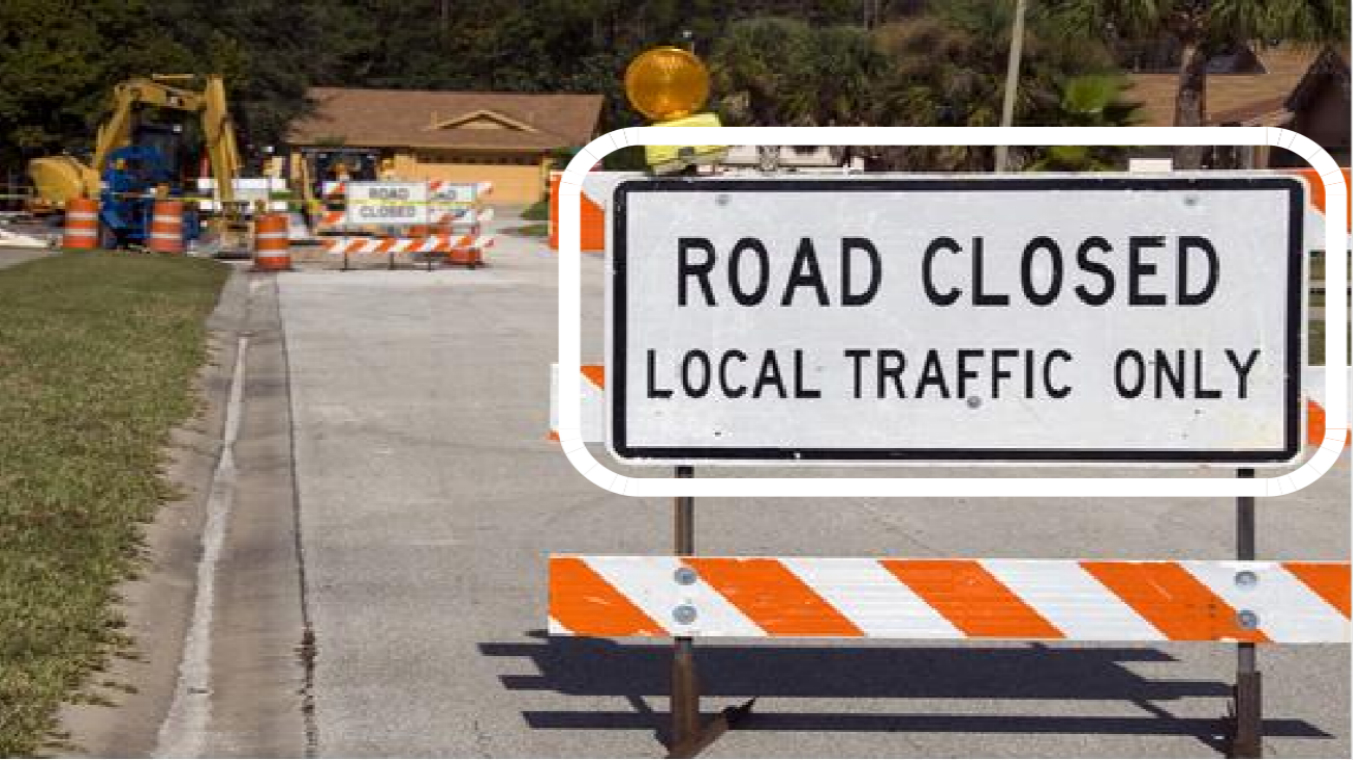
\includegraphics[width=\linewidth]{Figs/RTDrive/motivation/local_traffic.jpeg}
    \vspace{-0.2cm}
    \caption{Instruction with complex semantics.}
    \label{motivation:local_traffic}
  \end{subfigure}%
 \begin{subfigure}[t]{0.33\textwidth}
    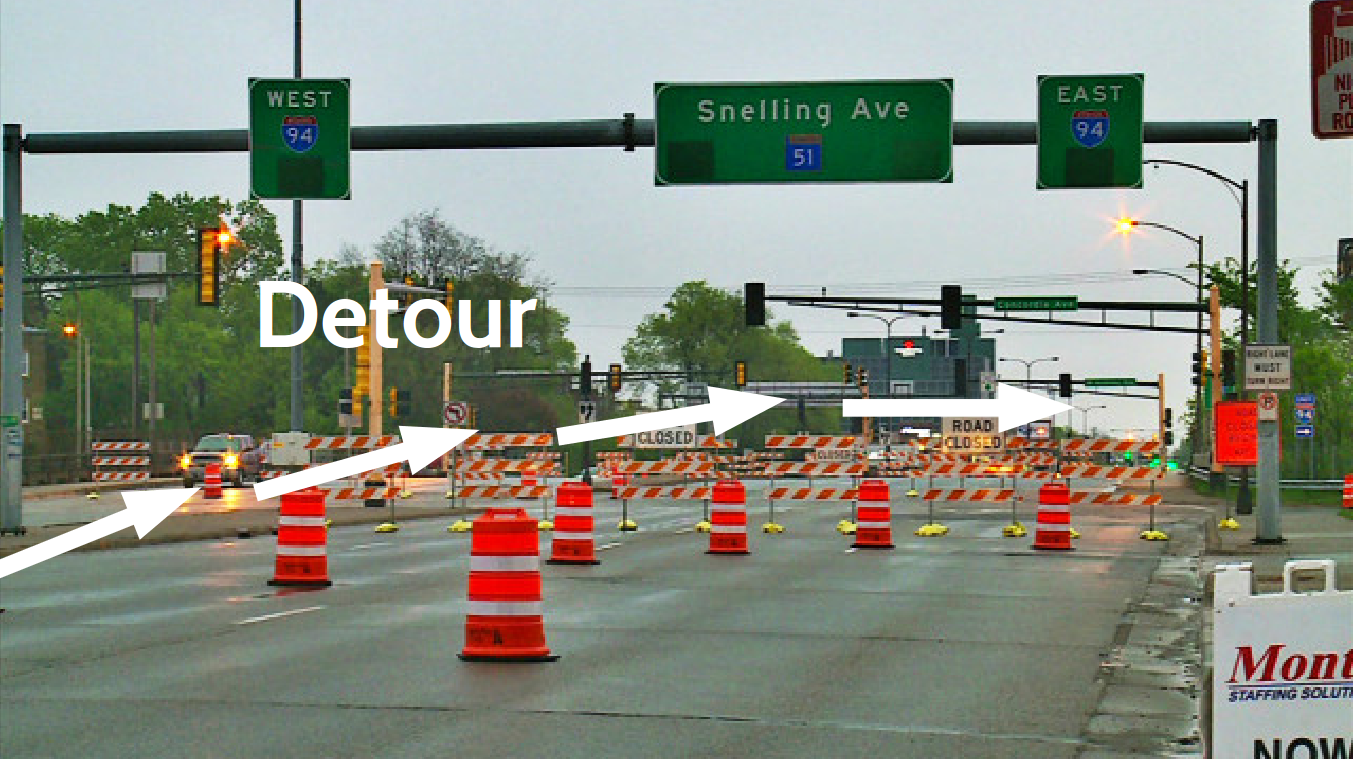
\includegraphics[width=\linewidth]{Figs/RTDrive/motivation/detour.jpg}
    \vspace{-0.2cm}
    \caption{Confusing detour arranged by barrels.}
    \label{motivation:detour}
  \end{subfigure}%
  \begin{subfigure}[t]{0.33\textwidth}
    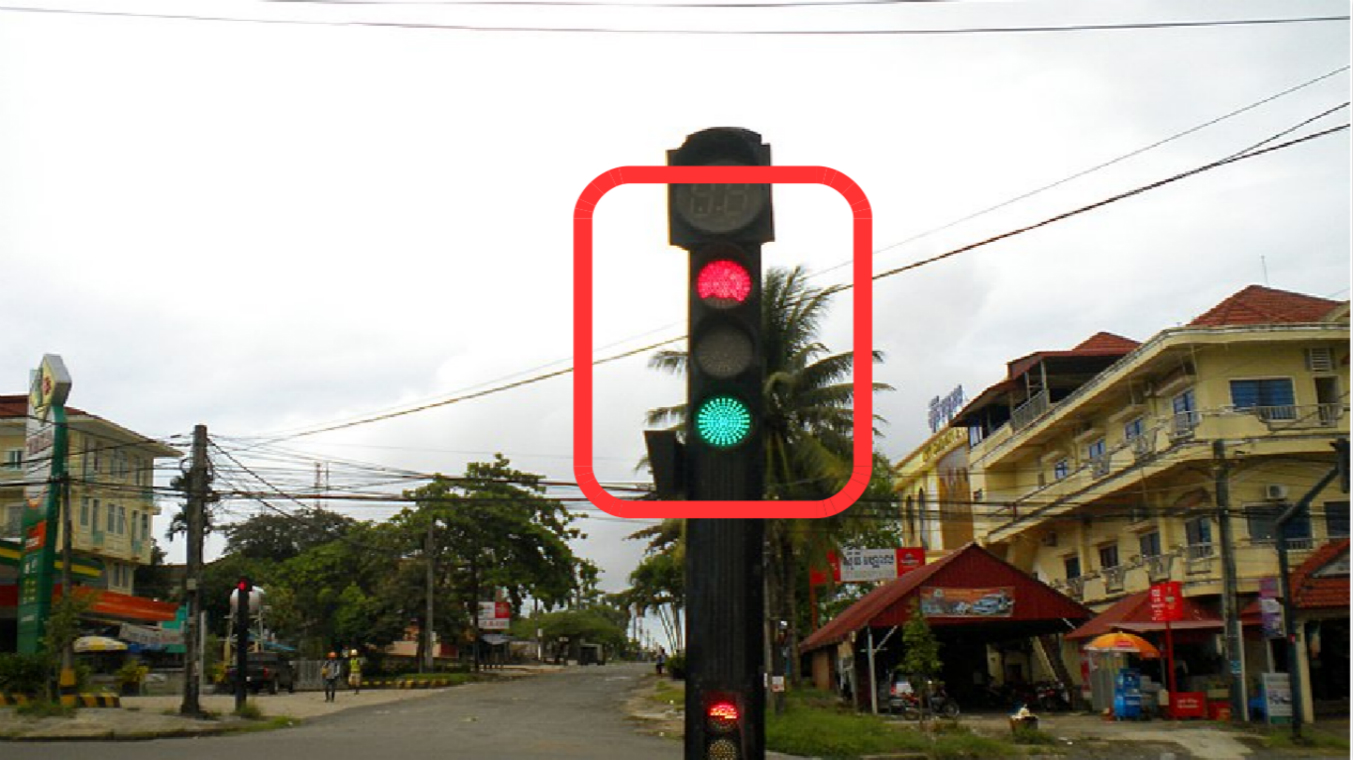
\includegraphics[width=\linewidth]{Figs/RTDrive/motivation/malfunctioning_traffic_light.jpg}
    \vspace{-0.2cm}
    \caption{Malfunctioning traffic lights.}
    \label{motivation:malfunction}
  \end{subfigure}%
  \vspace{-0.3cm}
  \caption{Self-driving system may occasionally fail under diverse real world conditions.}
  \label{motivation}
  \vspace{0.0cm}
\centering
\end{figure*}


\subsection{Self-Driving System Overview}


A self-driving system consists of several modules that are responsible for
different functionalities, i.e.,  
perception, localization, planning and control \cite{pendleton2017perception}. 
Perception refers to the ability to collect information and extract
relevant knowledge from the environment, 
such as detecting obstacles, identifying lane markers,
and categorizing these data by their semantic meanings. 
Localization refers to the ability to determine the 
vehicle's position with respect to the environment. 
Planning refers to the process of making purposeful decisions 
in order to navigate the vehicle 
while avoiding obstacles and optimizing over designed heuristics.
Finally, a control module is used to execute the planned actions.
Similar to human drivers, self-driving vehicle follows predefined traffic rules, 
such as drive within lane, do not cross double yellow line (except left turns),
stop at the red traffic light (except right turns in certain cases) etc. 
The perception module is used to understand the environment 
and traffic rules. 
If the perception module fails to do so, the vehicle may try to park
safely or operate with undefined actions \cite{waymo}.  

\subsection{Self-Driving System Failure Analysis}
\label{sec_failure}

We present several challenge conditions that a self-driving system
may fail if such conditions are not considered at system
design time. 


\textbf{Road sign or instruction with complex semantics}. 
The road sign or instruction can be too complex to be 
understood by self-driving system. 
One such example is illustrated in Fig. \ref{motivation:local_traffic}, 
where the road is closed and only local traffic is allowed. 
The self-driving system could fail to understand 
the semantics of ``local traffic'' or
fail to understand if it belongs to ``local traffic''.
Other complex semantics of instructions include
specific dates, specific type of vehicles 
and street names. 
If the self-driving system cannot understand road sign 
or instruction, it needs further human input. 


\textbf{Confusing and complex detour}.
Confusing detour due to misplaced cones or complex instructions 
may cause self-driving system failure. 
As shown in Fig. \ref{motivation:detour}, an experienced driver
can follow the barrels and drive out of the road boundaries
to pass this area, while a self-driving system may 
fail to identify a detour. 
Since there is no specific rules to place
traffic barrels, it is hard to find a general logic to 
learn where the detour is. 
There are also detour instructions that specify the street
name, exit number, special event instructions, 
that are too complex to be handled
by self-driving systems.
In such conditions, human knowledge and inputs are required. 

\textbf{Confusing or malfunctioning traffic lights/signs}.
Malfunctioning traffic light may cause self-driving
system failure as well. 
One example is shown in Fig. \ref{motivation:malfunction}, 
the traffic light turns to both red and green, 
and the self-driving system may fail to understand 
the traffic light is malfunctioning and act
with undefined behaviors.
Accidents may happen if all the traffic lights turn green at
an intersection.  
There are also confusing traffic light (e.g., yellow left turn light etc.)
and road signs (e.g., no right turn on red etc.) that
could need human inputs
\footnote{\url{https://www.youtube.com/watch?v=femUe6bds0U}}. 



\textbf{Perception failure at night and more}
Visibility and weather conditions are challenging for self-driving 
systems as well, 
i.e., low visibility due to fog \footnote{\url{https://www.youtube.com/watch?v=uYav3_7miIc}},
lane markers are covered by snow
\footnote{\url{https://www.youtube.com/watch?v=fc0yYJ8-Dyo}}.
There are also other conditions that are so complex
that a computer system may fail to handle, such as 
LIDAR or camera failures \cite{waymo}.


\subsection{Remote View and Control}


\begin{figure}[t]
\centering
\vspace{-0.2cm}
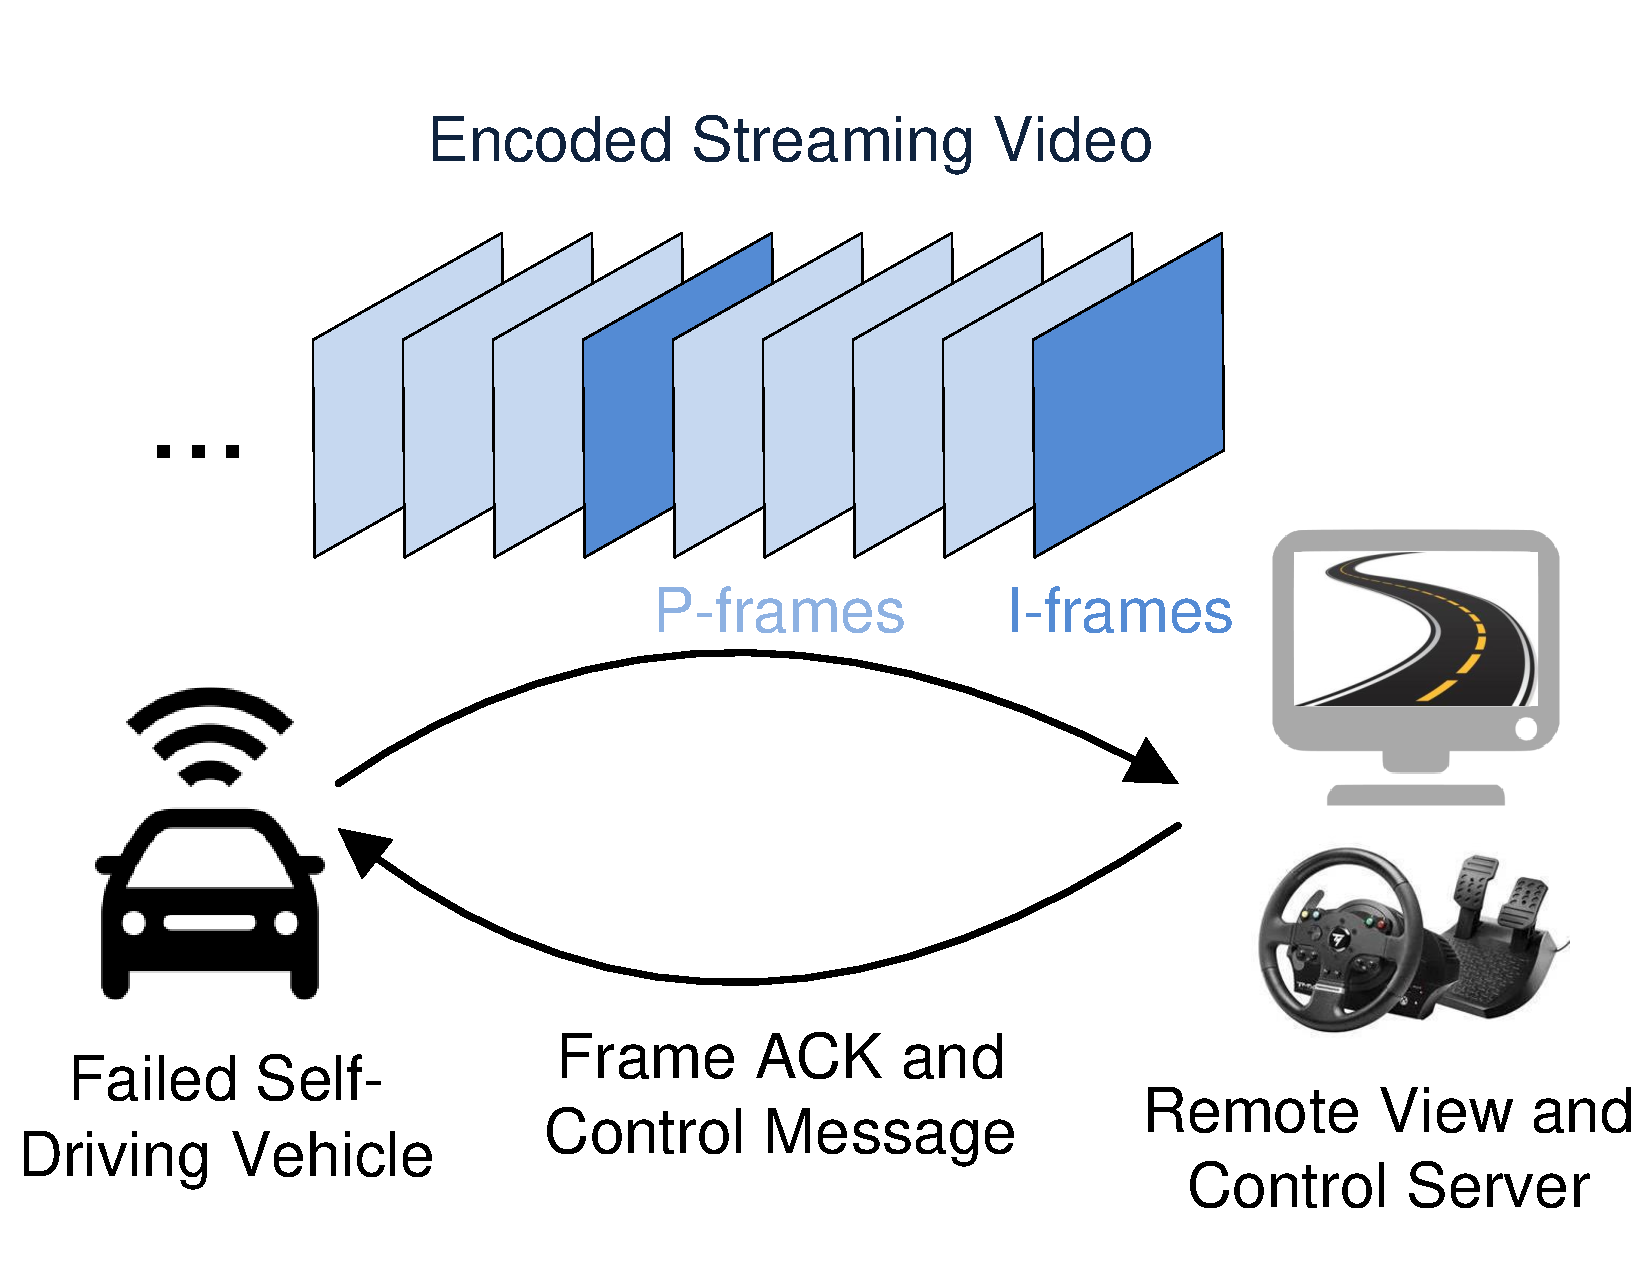
\includegraphics[width=2.6in,angle=0]{Figs/RTDrive/illustration.pdf}
\vspace{-0.4cm}
\caption{Remote view and control server to augment self-driving systems
(only when the self-driving system fails).}
\vspace{-0.4cm}
\label{illustration}
\centering
\end{figure}

With the possibility of failure in the complex road or traffic
conditions, remote view and control systems can act as a safe backup
of self-driving systems, 
i.e., the view and control can be transferred to the remote
operator upon these occasional failures describe in section \ref{sec_failure}. 
It also releases the human drivers behind the wheel who take over the 
control after system failures \cite{waymo}. 
A high level architecture is illustrated in Fig. \ref{illustration}.  
Upon system failure, the view of self-driving vehicle
is sending to the remote server, 
and the operator can view and control the vehicle in real time. 
Suppose a road lane is closed due to road work, 
a self-driving system can simply detect
that the current lane is blocked,
while it may fail to understand the semantic meanings
of the road signs. 
The remote human operator can take over the control and 
return the control to the self-driving system once the vehicle pass this road segment. 
Our work focus on the design of video encoding and live streaming protocol
in this application scenario. 
Our live streaming experiments are conducted with video streams
collected in real world driving trips, 
and the remote control experiments conducted with customized 
radio control vehicle in lab environment. 
The implementation and experiment on a real self-driving vehicle 
is left for future work. 







\section{The Design of RTDrive}




\begin{figure}[t]
\centering
  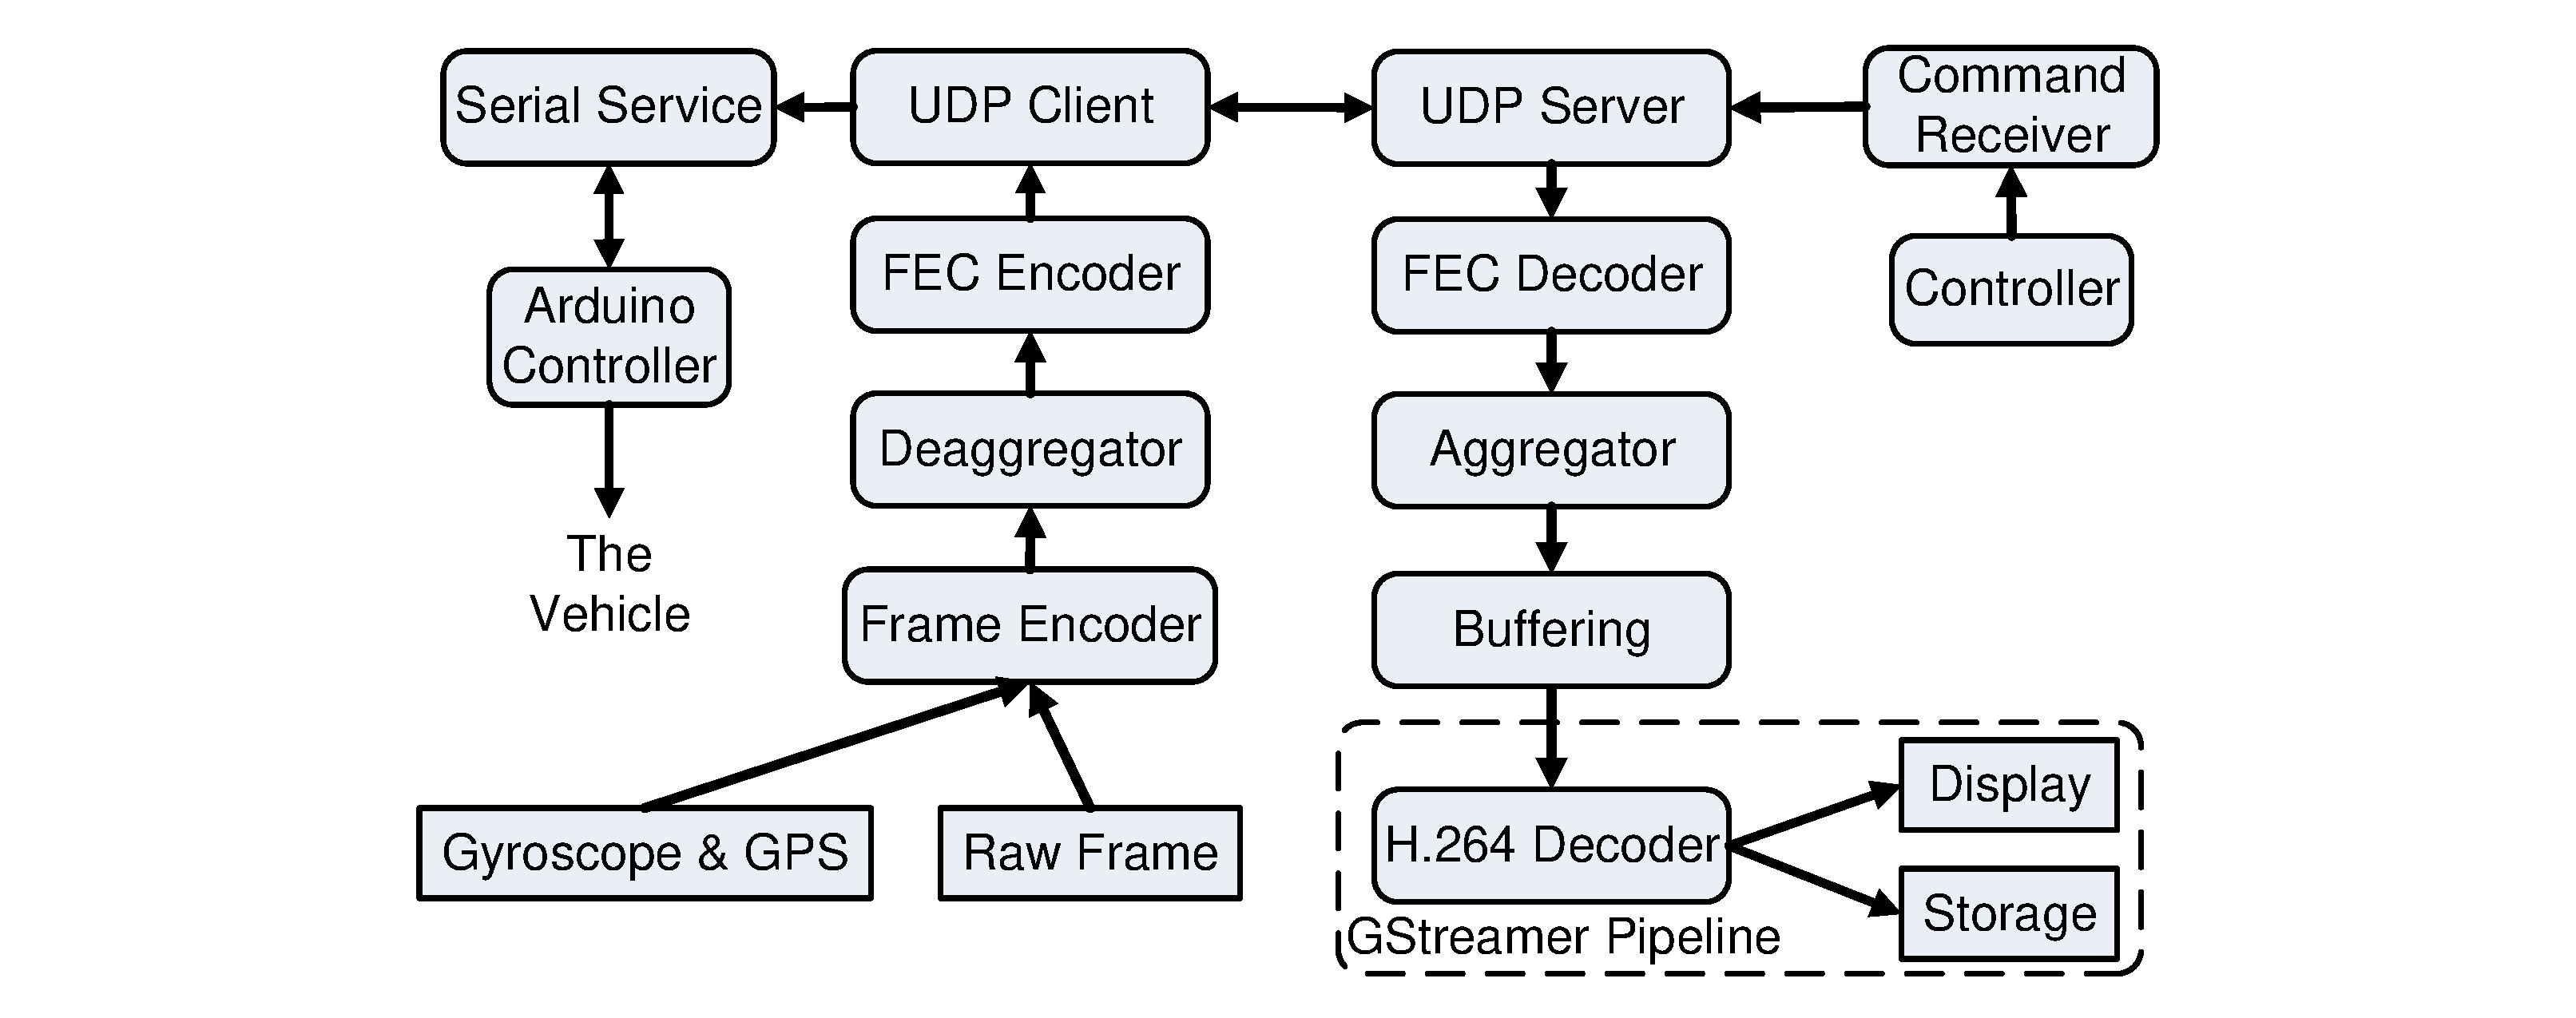
\includegraphics[width=3.4in,angle=0]{Figs/RTDrive/architecture.pdf}
\caption{The architecture of the live streaming and control system.}
\vspace{-0.5cm}
\label{server}
\end{figure}

RTDrive consists of an Android live streaming system and 
a remote control server. 
The architecture of the Android live streaming system is illustrated
in Fig. \ref{server}. 
The client side consists of two pipelines, the live streaming pipeline and the self-driving
pipeline. 
The live streaming pipeline includes context-aware video encoding, frame
deaggregation and FEC encoding.  
It encodes the video and streams to the remote server through transportation
protocols (details in section \ref{sec_udp_tcp}). 
The self-driving pipeline consists of object detection and lane marker detection. 
In the cases there is blockage in the lane, or no lane boundary is detected,
the control is transferred to remote server. 
while implementation of a fully self-driving vehicle
is out of the scope of this work, 
we present a framework that can be extended to a fully self-driving system, 
The architecture of the remote control server is illustrated in Fig. \ref{server}. 
It consists of two pipelines as well. 
A control pipeline is used to receive the control command from
an Android controller and then send to the vehicle. 
A video display pipeline is used to decode the frame packets
and display the streaming video to the operator. 



\begin{figure*}[ht]
  \begin{subfigure}[t]{0.32\textwidth}
    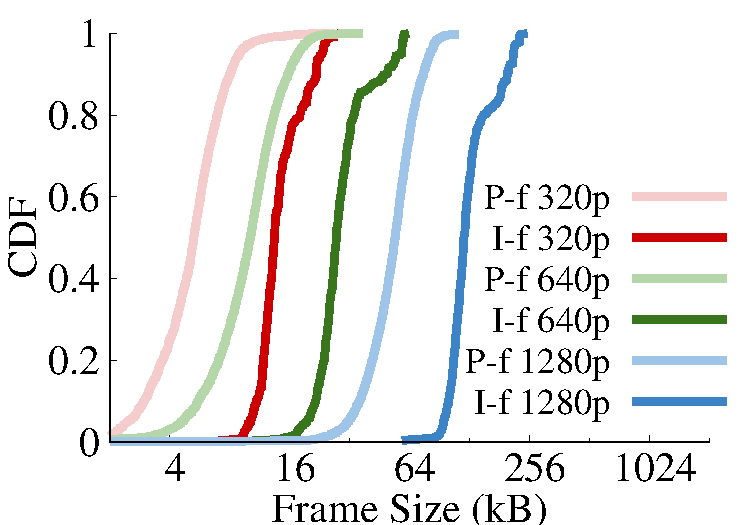
\includegraphics[width=\linewidth]{Figs/RTDrive/I_P_frame_size.pdf}
    \caption{The size distribution of I-frames and P-frames under three different resolutions and bitrates.}
    \label{frame_size}
  \end{subfigure}
\hspace{0.3cm}
  \begin{subfigure}[t]{0.32\textwidth}
    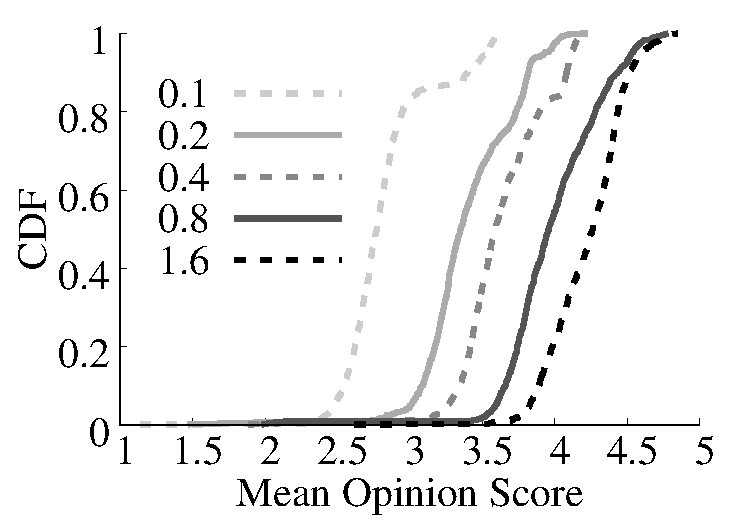
\includegraphics[width=\linewidth]{Figs/RTDrive/video_bitrate_quality.pdf}
    \caption{Video quality under different video bitrates (unit: mbps).}
    \label{bitrate_quality}
  \end{subfigure}
\hspace{0.3cm}
  \begin{subfigure}[t]{0.32\textwidth}
    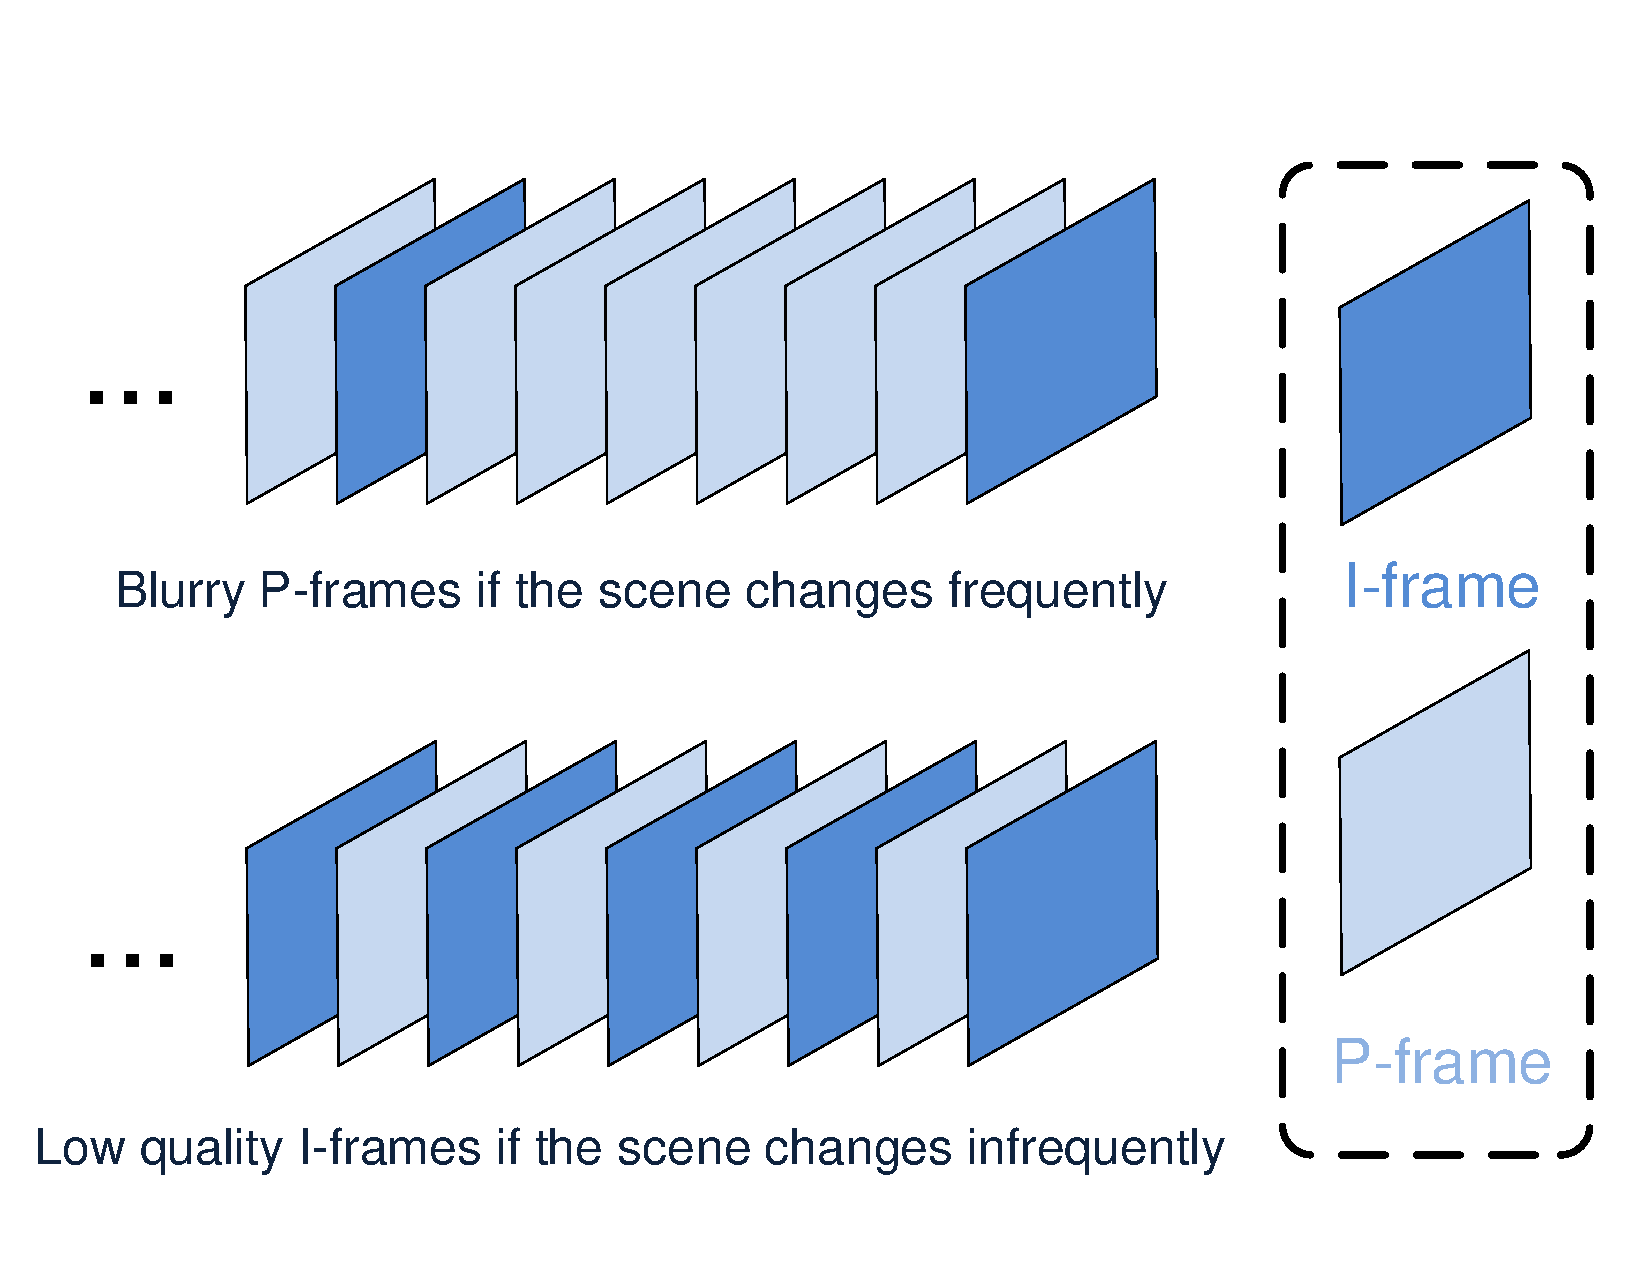
\includegraphics[width=\linewidth]{Figs/RTDrive/intervals.pdf}
    \caption{Illustration of I-frame interval and video quality.}
    \label{interval}
  \end{subfigure}
\caption{Video encoding and image quality.}
\end{figure*}


\subsection{Context-Aware Video Encoding}


Video encoding is a process that compress the raw video frames 
into frames of less sizes 
\footnote{Video/frame encoding is equivalent to video/frame compression 
and we use them interchangeably in this chapter}.
In this section, we present the overview of frame encoding, 
the relation between video encoding bitrate and video
quality, and how we can utilize
vehicle dynamics to improve video encoding efficiency.  

\subsubsection{Frame Encoding}
\label{sec_frame_encoding}




A video is a time series of video frames, or images. 
The size of each frame depends on the resolution and pixel encoding method. 
For example, for a frame of $w * h$ resolution, and each pixel 
is encoded by 3 bytes, i.e., 
one byte for each color of red, green and blue,
the total size of this frame is $3 * w * h$ bytes. 
For a frame with resolution of $640*480$, 
the size of one frame is around 1 Megabyte. 
The number of frames in one second is called frame rate. 
Suppose we send video streaming at 10 frames per second, 
we need a bandwidth of 100Mbps, which is too large to
be handled by today's wireless networks. 
Video streaming applications uses frame encoding techniques
to reduce the size of the frames. 
One frame can be compressed itself by using the statistical 
properties of image data. 
Continuous frames can be compressed by extracting the 
difference among video frames. 
The frame compression techniques can be lossless and lossy. 
Live streaming applications usually use lossy compression 
for its higher compression ratio. 


We compress the video by using video compression standard 
H.264 or MPEG-4 \cite{marpe2006h}.
In H.264, there are two types of frames, 
I-frame and P-frame. 
An I-frame, or Intra-coded frame, is a complete image. 
P-frame (Predicted frame)  
hold only the part that changes between frames.
The size distribution of I-frames and P-frames
under various resolution is illustrated in Fig. \ref{frame_size}. 
The three resolutions of 320x240, 640x480 and 1280x960, 
are set with bitrate 0.5Mbps, 1Mbps and 4Mbps, respectively. 
The size of I-frames and P-frames depends on 
the video encoding bitrate. 
If we use the same bitrate for two different resolutions, 
the frame sizes are similar but the quality will
be different (the relation between bitrate and video quality is
discussed in section \ref{sec_quality}). 
The median size of I-frames is 2-4 times larger
than that of P-frames in different resolutions. 
In other streaming applications, 
it can also use both previous and forward frames 
to generate B-frame (Bidirectional predicted picture) 
to better compress the frame.
B-frame is not used for live streaming as it requires
to stream the frame at the earliest possible time. 



The I-frame interval is defined as the time between 
two continuous I-frames and it is usually 1-5s \cite{zhang2012profiling, yu2014can}. 
The frame rate ranges from 1 to 15 in popular VoIP 
applications such as Skype \cite{zhang2012profiling} and Google Hangout \cite{yu2014can}. 
The server decompresses the video frame by using GStreamer pipeline \cite{gstreamer} 
and sends back the timestamp associated with the frame 
(the details are discussed in section \ref{streaming_protocol}). 


\subsubsection{Video Quality}
\label{sec_quality}


We use Blind and Referenceless Image Spatial Quality Evaluator (BRISQUE) 
\cite{mittal2012no} and Mean Opinion Score (MOS) \cite{bauman2017towards}
to evaluate the video/frame quality. 
The video quality is shown as a cumulative distribution function of frame qualities.  
BRISQUE trains a model using identical predictable statistical features, 
called natural scene statistics (NSS). 
NSS are based on normalized luminance coefficients in the spatial domain, 
and are modeled as a multidimensional Gaussian distribution. 
Distortions appear as perturbations to the Gaussian distribution.
It has been shown that these features correlate well with 
human judgements of quality \cite{mittal2012no, bauman2017towards}. 
The function uses the NSS features and corresponding opinion scores to train
a support vector machine regression model. 
The correlation between BRISQUE and MOS is summarized in Table \ref{brisque}.
It maps the score of one frame (0-100) calculated by BRISQUE to 
a MOS between 1 and 5. 
We use MOS as the only metric to evaluate frame quality. 

The video of one resolution can be encoded into different bitrates. 
High bitrate leads to high quality video. 
We compress a video with different bitrates (1kbps to 2mbps) and evaluate the video qualities.
The results are shown in Fig. \ref{bitrate_quality}. 
The bitrates of lower than 0.1mbps and higher than 1.6mbps are not shown 
in the plot. 
There are 1 I-frame within 10 frames 
and the 10\% of the frames with higher quality are mainly I-frames.  
Encoded video with lower than 0.1mbps downgrades the video quality marginally
comparing with the video with 0.1mbps. 
Similarly, encoded video with higher than 1.6mbps improves the
video quality marginally comparing with the video with 1.6mbps. 
Within the bitrate range of 0.1mbps and 1.6mbps, 
it roughly need to double the bitrate to improve the video quality linearly. 
We refer video encoding efficiency as the median video quality under
same encoding bitrate or the bitrates required to achieve the same
median video quality. 



\begin{table}[t]
  \centering
  \caption[psnr]{BRISQUE vs MOS}
  \vspace{-0.0cm}
  \label{brisque}
  \begin{tabular}{|c|c|c|c|c|c|}
  \hline
BRISQUE & 90 & 72 & 54 & 36 & 18
\\  \hline
MOS & 1 & 2 & 3 & 4 & 5
\\  \hline
Video Quality & Bad & Poor & Fair & Good & Excellent 
\\  \hline      
  \end{tabular}
  \vspace{-0.0cm}
\end{table}


\subsubsection{Context-Aware Encoding}


We present how to adjust video encoding parameters to improve
encoding efficiency according to vehicle dynamis in this section.
Suppose we use a fixed bitrate to encode a video, 
it is import to decide how many I-frames we want to encode. 
If the scene changes frequently, it needs more I-frames to reduce
the quality of each I-frame but increase the overall quality,
given the encoding bitrate is the same. 
If the scene changes infrequently, it needs less I-frames
to achieve a high encoding quality of I-frames 
as well as the P-frames since P-frames requires less data. 
An illustration is shown in Fig. \ref{interval}.
Our context-aware encoding technique utilizes this 
intuition to improve the overall video encoding efficiency
by sensing vehicle dynamics. 
The basic idea is to increase the I-frame interval at lower
speed and decrease it at higher speed or during steering events. 


To track the vehicular speed and angular velocity, we use
the GPS and the gyroscope sensor. 
The gyroscope is used to track 3D angular velocity of the 
smartphone. 
Interested readers can refer to \cite{wang2013sensing, chen2015invisible}
for how to use gyroscope to track vehicle steering events. 
The pseudo code of the context-aware encoding algorithm 
is shown in Algorithm \ref{contextaware}.
The $timestamp\_$ tracks the timestamp of last frame. 
the $gps\_$ and $gyro\_$ track the GPS data and gyroscope data 
recorded in last function call, respectively.
The $dist\_$ and $deg\_$ are the accumulated distance
and degree the vehicle travelled, respectively.
The $check\_$ refers to the checkpoint where last I-frame is created.
The algorithm checks the accumulated distance, angles and time
to decide if next frame should be I-frame or P-frame. 

%\begin{enumerate}
  \begin{algorithm}[t]
   \caption{Check if I-frame is required by sensing vehicle dynamics}
    \label{contextaware}
    \begin{algorithmic}[1]
\Function{requireKeyFrame}{$gps, gyro$}
  \State $now = currentTimeMillis()$
  \State $init = false$
  \If {$timestamp\_ == -1$}
    \State \Return $init = true$
  \Else
    \State $dur = now - timestamp\_$
    \State $dist\_ = dist\_ + gps\_.speed() * dur$    
    \State $deg\_ = deg\_ + gyro\_.angular() * dur$
  \EndIf
  \State $timestamp\_ = now$
  \State $gps\_ = gps$
  \State $gyro\_ = gyro$
  \If {$init || dist\_ >= \theta_{dist} || deg\_ >= \theta_{degree} || now - check\_ >= \theta_{t}$}
    \State $dist\_ = 0$
    \State $deg\_ = 0$
    \State $check\_ = now$
    \State \Return $true$
  \Else
    \State \Return $false$
  \EndIf
\EndFunction
\end{algorithmic}
\end{algorithm}
%\end{enumerate}



\subsection{Live Streaming Protocol}
\label{streaming_protocol}


We present the design of live streaming protocol in this section. 
We discuss different protocol design choice and present a consistent-latency
view when displaying live streaming video to remote operator. 
Measuring the performance of live streaming applications, such as 
Skype \cite{zhang2012profiling} and Google Hangout \cite{yu2014can}, 
is a active research topic. 
The implementation and application scenario differentiate us from
these measurement studies. 


\subsubsection{UDP or TCP}
\label{sec_udp_tcp}

Existing VoIP applications rely on UDP extensively, 
i.e., Skype \cite{zhang2012profiling} and Google Hangout \cite{yu2014can}.
Google Hangout uses UDP by default and switch to TCP if UDP traffic 
is blocked. 
Comparing with TCP, UDP is connectionless, does not have 
congestion control and retransmission mechanisms. 
In TCP, if one packet of a frame gets lost, 
packet frame will be re-transmitted and 
the frame is delayed for an entire RTT. 
In UDP, if one packet of a frame gets lost, 
the rest of the frame can be displayed and 
it does not introduce extra latency. 
Therefore, UDP is a better choice for live streaming
applications. 
However, if the UDP packet is lost, the video quality
will drop, 
so it usually comes with loss rate estimation and 
forward error correction mechanisms. 
In our framework, we implement both TCP and UDP
to understand and compare the performance difference.
In our UDP implementation, we use frame ACK 
mechanism to send back loss rate and bandwidth
estimation results to the live streaming system. 
The frame ACK is sent through the same UDP channel. 
We will discuss how to handle lost frame ACK
when estimating loss rate and bandwidth in section 
\ref{sec_lossrate} and \ref{sec_bandwidth}. 
In our TCP implementation, we use socket buffer size 
to estimate TCP transmission rate and adjust
video encoding rate at application layer. 
If there is packet loss in the network, the TCP connection
will reduce transmission rate and the application layer
will reduce video encoding rate. 


\subsubsection{Forward Error Correction (FEC)}
\label{sec_fec}

To improve the video quality upon packet losses, 
we introduce forward error correction (FEC) in our framework. 
Missing frame data may cause video distortion and flickering.
FEC, also known as eraser code, is widely used in wireless transmission \cite{yu2014can}
and reliable file storage \cite{plank2009performance}.
In FEC, each frame is encoded into $n$ packets of length $m$. 
Among the $n$ packets, the first $k$ packets are the raw data
of the frame, and the rest $n - k$ packets are encoded packets, 
i.e., each byte of the encoded packet is the linear combination 
of corresponding byte in the raw packets. 
Since each video frame has different size, $k$ and $n$ are 
different for different video frames. 
To encode and decode one frame, 
it requires the packets have the same length.
We use a reference packet length to estimate the $k$ first, 
and then assign each packet with equal length $sz / k$, 
where $sz$ is the frame size. 
In this case, we need at most $k$ bytes for the
padding of the last packet. 
It reduces the extra padding from $O(m)$ to $O(k)$ ($k$ is usually much smaller than $m$).  
In case of packet loss, $n - k$ packets are encoded as redundancy.
We define the redundancy ratio as $rr = (n - k) / n$. 
If any $k$ of $n$ packets are received at the receiver side,
then the frame can be recovered. 

\subsubsection{Loss Rate Estimation}
\label{sec_lossrate}

To decide how many packets to encode, we need to track
the loss rate of the UDP transmissions. 
On the server side, we calculate frame packet loss rate. 
To determine the number of data packets $k$ and that of coded packets $n$
to be included in a given frame, we
calculate the effective loss rates $L$ after the diversity combining at
the server. 
In our framework, each frame has an unique frame identifier, 
and each frame is encoded into $n$ packets. 
Each packet has a unique index ranging from $0$ to $n - 1$. 
The first $k$ packets contains the raw data and the rest
contains the encoded redundancy.
The server side maintains a running frame identifier to record
current buffered packets. 
The server only buffer the packets of current frame, 
and if there is enough packets are received then
any future encoded packets of this frame is dropped. 
%The FEC packet buffering algorithm is listed in Algorithm \ref{fec_buffer}. 

\subsubsection{Bandwidth Estimation}
\label{sec_bandwidth}

Bandwidth is an important parameter for the video encoding algorithm
to decide which bitrate to use. 
If the video bitrate is larger than the bandwidth, 
the latency will be increased and the video may freeze.  
The video encoding algorithm can adapt the video bitrate
based on bandwidth measurement for better video quality 
and user experience. 
Similar to loss rate estimation, the connection bandwidth is estimated
at the server side as well. 
The bandwidth estimator divides time into equal intervals and 
estimate the loss rate in each interval. 
We estimate bandwidth based on interval instead of frame.
Because the packets in one frame may come in batch, 
and the bandwidth is overestimated if we just calculate
the bandwidth according to current frame. 

\subsubsection{Consistent-Latency View (CLV)}
\label{sec_clv}

%\begin{enumerate}
  \begin{algorithm}[t]
   \caption{Consistent-Latency View Buffering Algorithm}
    \label{algorithm_clv}
    \begin{algorithmic}[1]
\Function{consistentLatencyDisplay}{$frame$}
  \State $counter = counter + 1$
  \State $now = currentTimeMillis()$
  \State $diff = now - frame.sendTime$
  \If {$counter > 1 \&\& diff > \delta{t}\_$}
    \State $deviation = diff - \delta{t}\_$
    \State $\sigma{t}\_ = \beta{t} * deviation + (1 - \beta{t}) * \sigma{t}\_$
  \EndIf
  \If {$counter == 1$}
    \State $\delta{t}\_ = diff$
  \Else
    \State $\delta{t}\_ = \alpha * diff + (1 - \alpha) * \delta{t}\_$
  \EndIf
  \State $delay = (\delta{t}\_ + \sigma{t}\_) - diff$
  \If {$delay > 0$}
    \State $sleep(delay)$
  \EndIf
  \State $sendFrameToDisplay(frame.payload)$
  \State $storeFrame(frame)$
\EndFunction
\end{algorithmic}
\end{algorithm}
%\end{enumerate}



Each frame suffers different latencies over the wireless 
networks and the Internet. 
We usually experience discontinuous video display, 
where one frame may freeze for seconds and then go
faster than normal. 
We introduce consistent-latency view to
reduce video skipping and lagging. 
As shown in Algorithm \ref{algorithm_clv}, we track the time difference between 
the time the server receives the frame 
and the time the client sends out
the frame, $t_d = t_s - t_c$. 
$t_d$ also refers to the time difference between the server and client.
We use exponential average to model the average time 
difference $\sigma{t}\_ = \alpha * \sigma{t}\_ + (1 - \alpha) * t_d$, 
where $\alpha$ is within $[0, 1]$. 
Beside time difference, we also track the deviation 
of the time difference when the time difference is 
higher than the average, $\sigma{t}\_$. 
The average of the deviation is calculated as
$\delta{t}\_ = \beta * \delta{t}\_ + (1 - \beta) * t$, 
where $\beta$ is within $[0, 1]$.
To enable consistent-latency view, the frames are buffered based
on their arriving time. 
If the arriving time of one frame is earlier than expected, 
then it is buffered until $t_d$ is equal to $\sigma{t}\_ + \delta{t}\_$. 
If the arriving time of one frame is later than expected, 
it is sent to GStreamer display right away. 
This mechanism leads to higher average latency but 
lower latency deviation,
which reduces freezes and leads to smoother video streaming. 


\subsection{Self-Driving Module}

We design and implement an Android-powered self-driving module, 
where the system can identify lane boundaries, objects and
and potential blockage. 
The lane boundaries are identified by Canny edge detector
\cite{canny1987computational} and some heuristics of 
using lane colors. 
In our detector, we search on both sides by starting from the 
middle of the pixel columns, the lane boundaries are detected if there are
white/yellow edges detected.
The objects the potential blockages are identified by using
Cascade classifier \cite{viola2001rapid}. 
Cascade classifier extracts and select features from cropped objects within images, 
and match the features with new images to identify the objects.    
Each feature is a subrectangle extracted from the image matrix. 
Each such subrectangle is represented by two or four values record 
the accumulated pixel value sum of the subrectangle.
A decision tree is used to select some key features from the massive
subrectangles. 
The design and implementation of an universal self-driving system is very
complex and out of scope of this work. 
Interested readers may refer to \cite{waymo, canny1987computational, viola2001rapid} for more
details on identifying objects towards building a fully self-driving vehicle. 

\nop{
\subsection{In-Lane Self-Driving}

We implement an Android-powered in-lane self-driving system, 
where the vehicle can navigate within lane boundries
and identify potential blockage. 
The design and implementation of an universal self-driving system is very
complex and out of scope of this work. 


\subsubsection{Blockage and Object Detection}


\begin{figure}[t]
\centering
\vspace{-0.0cm}
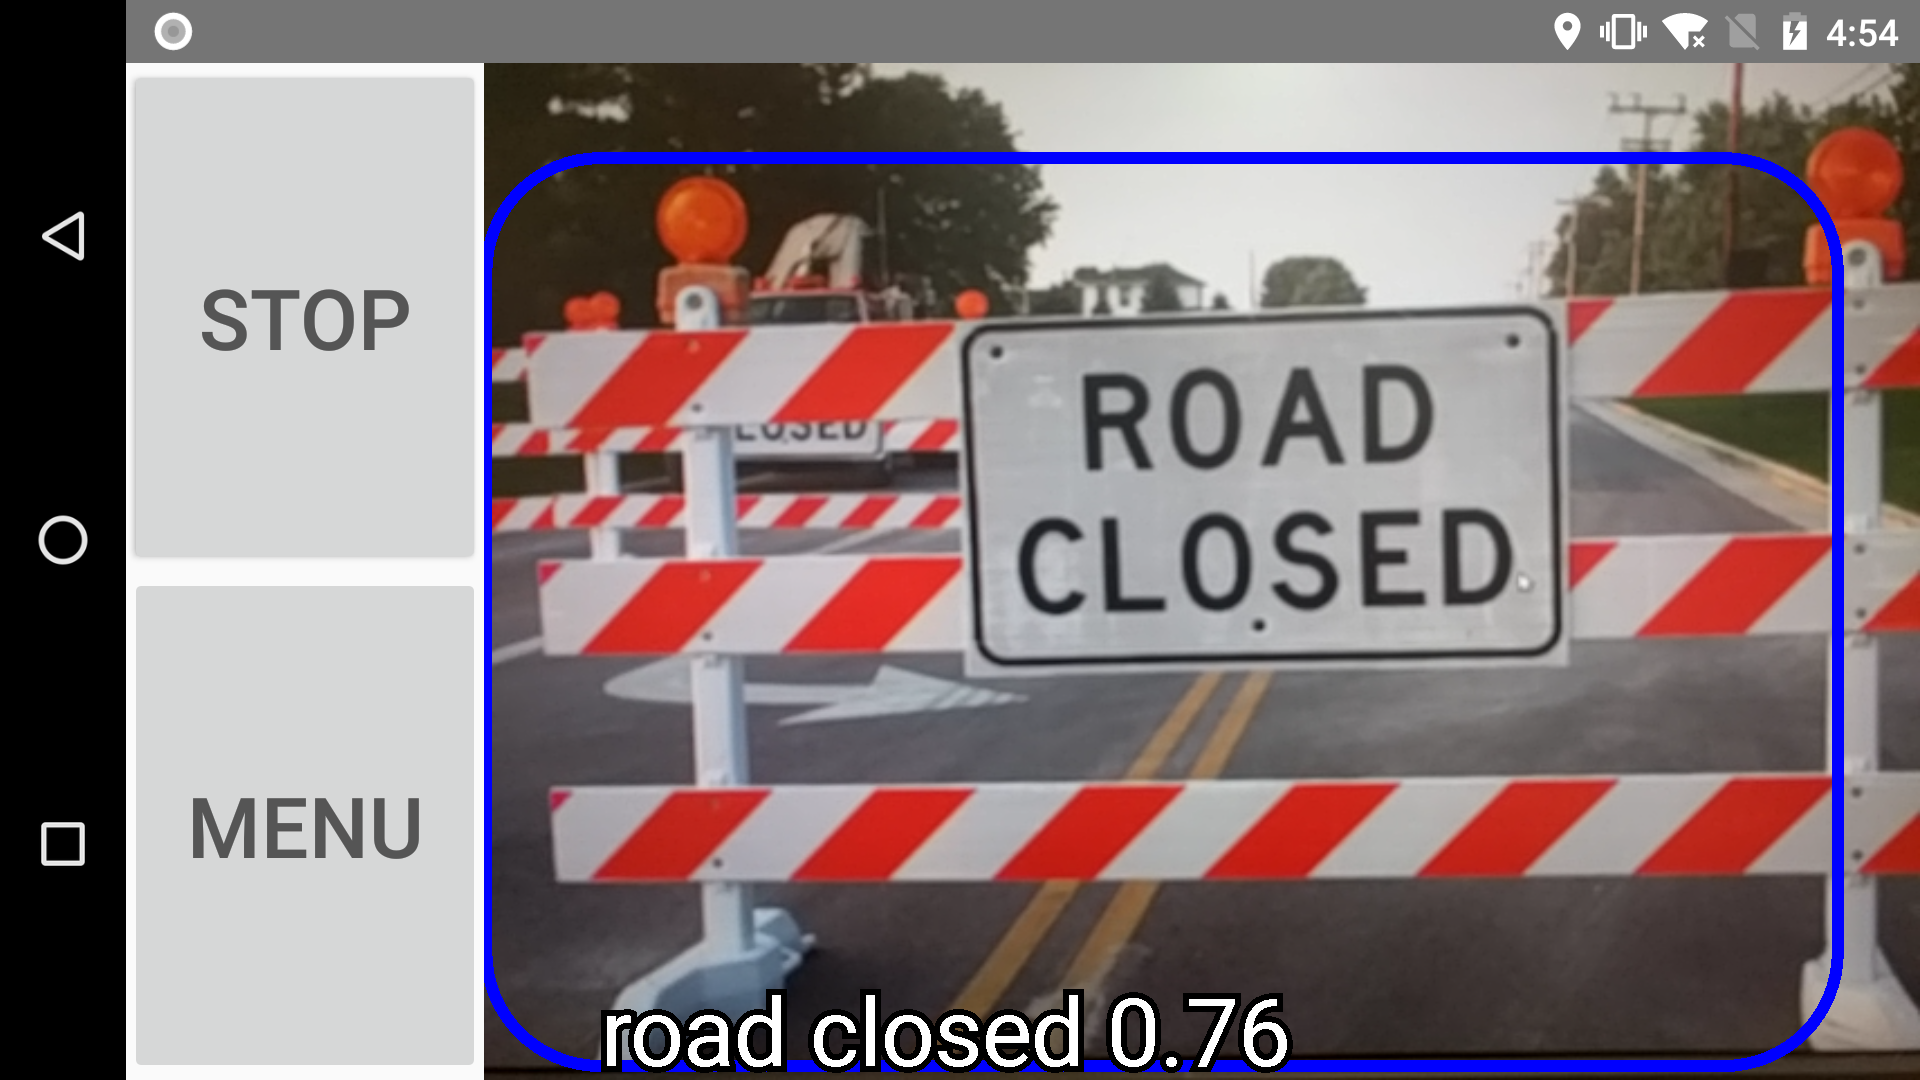
\includegraphics[width=2.6in,angle=0]{Figs/RTDrive/road_closed.png}
\vspace{-0.0cm}
\caption{Road blockage and object detection by TensorFlow in Android Camera Preview mode.}
\vspace{-0.2cm}
\label{road_closed}
\centering
\end{figure}

\begin{figure}[t]
\centering
\vspace{-0.0cm}
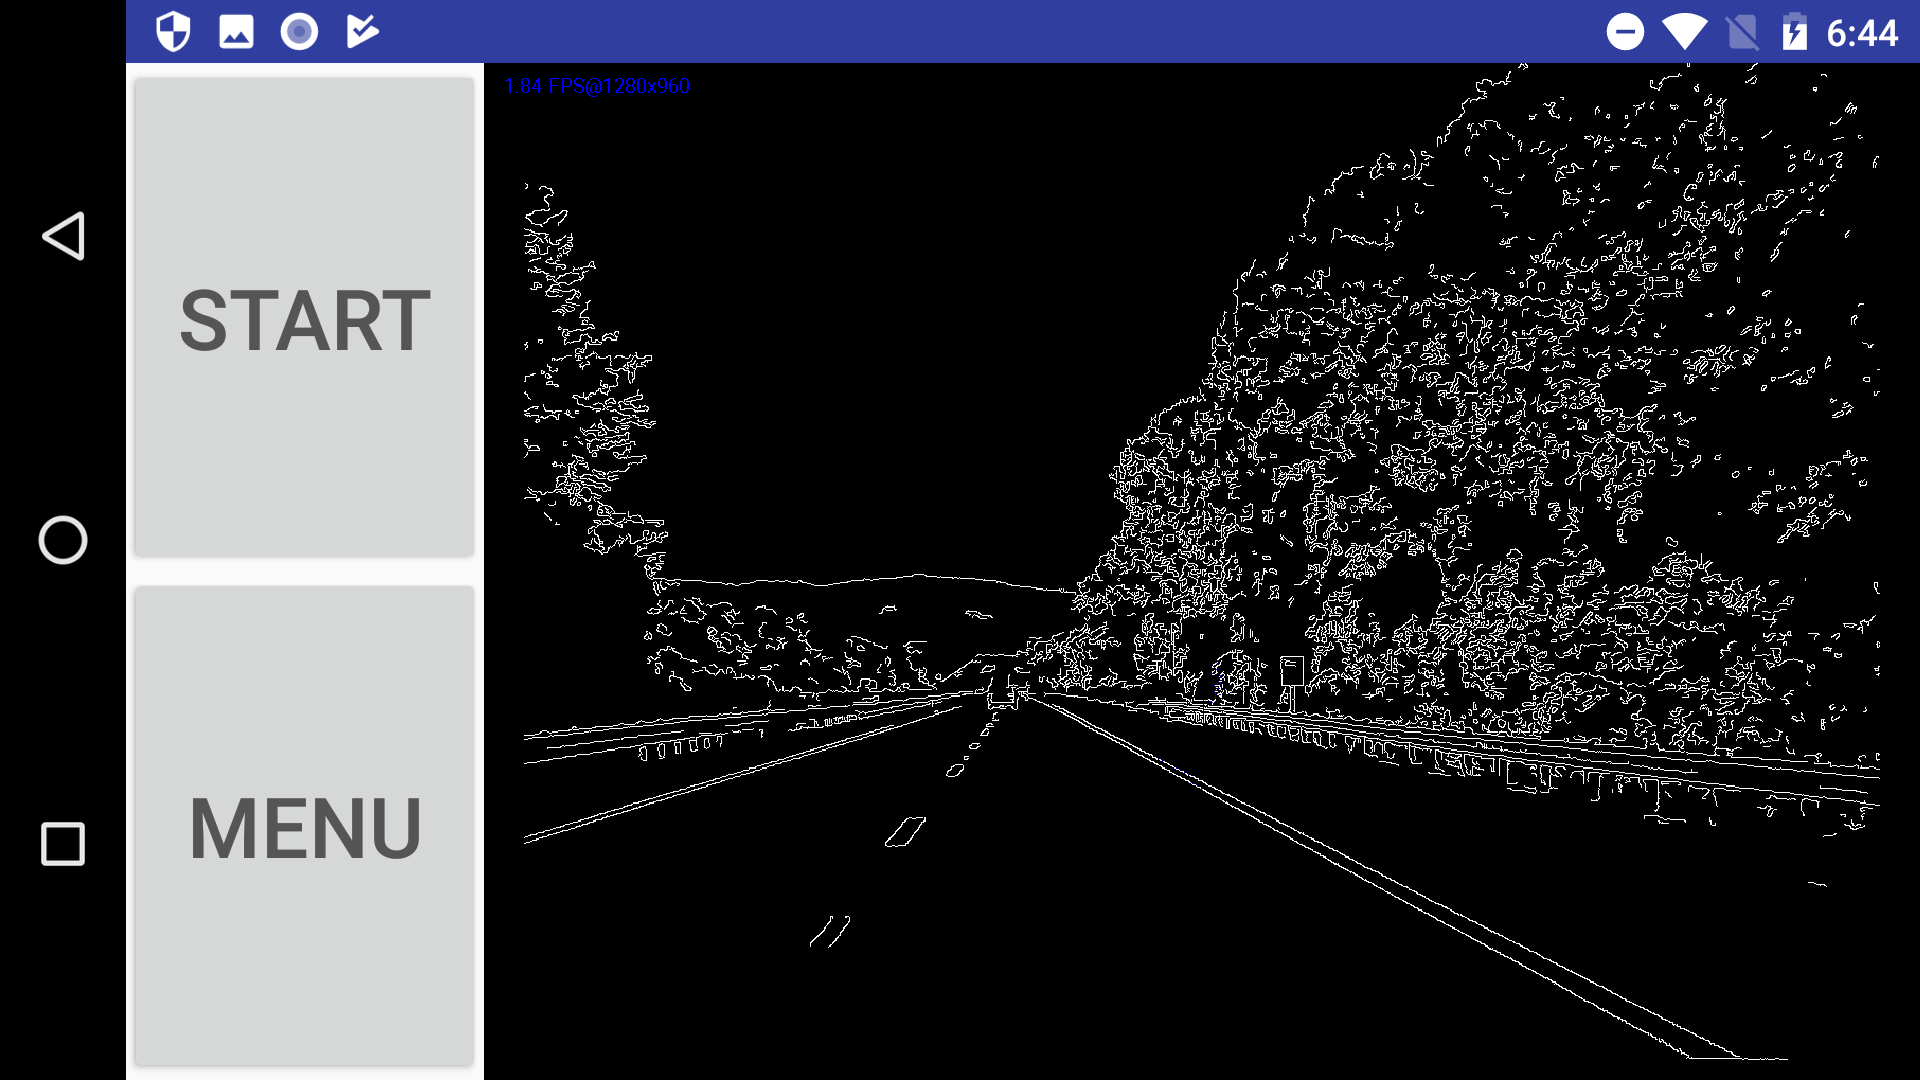
\includegraphics[width=2.6in,angle=0]{Figs/RTDrive/lane_markers.png}
\vspace{-0.0cm}
\caption{Lane marker and road boundary detection by using OpenCV Canny edge detector
in OpenCV preview mode.}
\vspace{-0.2cm}
\label{lane_marker}
\centering
\end{figure}

We use TensorFlow to detect objects and road blockage. 
TensorFlow Core programs consists of two discrete sections, 
building the computational graph and 
running the computational graph \cite{abadi2016tensorflow}.
A computational graph is a series of TensorFlow operations arranged into a graph of nodes. 
In this graph, each node takes zero or more tensors 
as inputs and produces a tensor as an output. 
Nodes in the graph represent mathematical operations, 
while the graph edges represent the multidimensional 
data arrays (tensors) communicated between them. 
Building the computational graph is to use labeled data 
to train the parameters of the graph, 
running the computational graph is to predict the 
outcome given the inputs. 
In our implementation, the computational graph is a blackbox, 
i.e., the input is the image data and 
the output is the identified object. 
We use a prebuilt computational
graph to identify objects and road signs. 
A ``road closed'' sign is identified in Fig. \ref{road_closed}
with a confidential value 0.76 
(higher value means stronger confidence, 1 means the best). 
If such a similar blockage is detected and the self-driving
system cannot handle, the control is transferred to the
remote operator.  
We refer interested
readers to \cite{abadi2016tensorflow, huang2016speed} for detailed graph tranning
and running in TensorFlow.


\subsubsection{Lane Marker and Road Boundary Detection}


We use Canny edge detector, 
Color detector and herustic algorithms to track lane markers and road boundaries. 
Canny edge detector is a multi-stage edge detection
algorithm. 
It uses Gaussian filter to smooth the image in order to remove the noise, 
and then finds the intensity gradients of the image to determine
all possible edges. 
The weak edges are removed if weak or not connected with strong edges. 
Canny edge detector helps us to find the lane and road boundaries. 
To determine the lanes, we use color detector to find all
white and yellow lanes, given the lane markers are either white
or yellow on most roads in US. 
The lane marker and road boundary detection is illusrated in Fig. \ref{lane_marker}. 


\subsubsection{Steering Angle Estimation}

To estimate the steering angle, we use a heuristic algorithm. 
There could be more than one lane in a road segment
and we also need to label the current lane of interest. 
We search from the center of the camera, assuming 
the camera is at the center of the car. 
The first lane markers on both the left side and right side
form the current lane. 
If the lane is straight, then the image view ends at a vanish point
that the lane markers of both side point to. 
The vanish point and the lane markers form a triangle. 
If the lane is curving, then the lane markers of either side
will deviate from this triangle. 
The steering angle is estimated by the coordinates difference
between the triangle and the curved lane markers.   

 }








\section{Implementation}



\begin{figure}[t]
\centering
  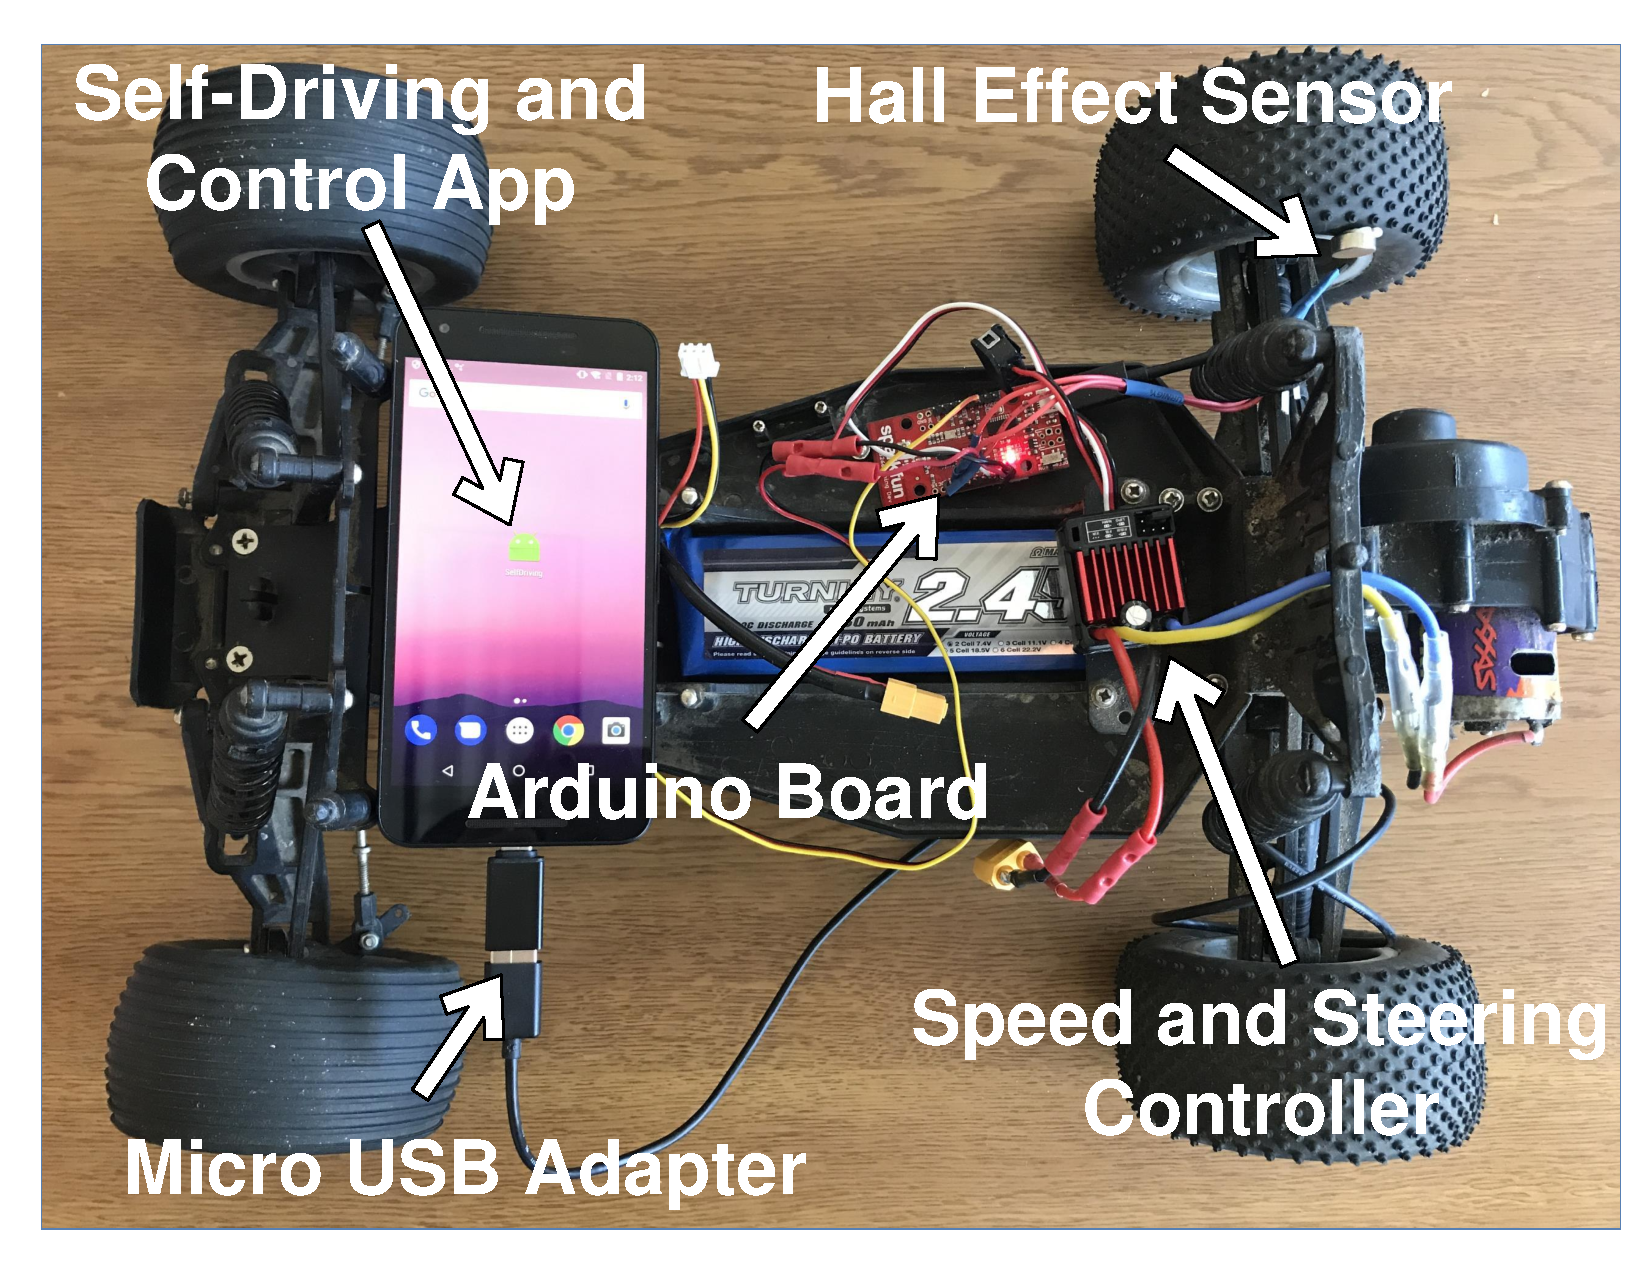
\includegraphics[width=2.4in,angle=0]{Figs/RTDrive/rc_car.pdf}
\vspace{-0.2cm}
\caption{The vehicle testbed.}
\vspace{-0.5cm}
\label{rc_vehicle}
\end{figure}

\begin{figure}[t]
\centering
  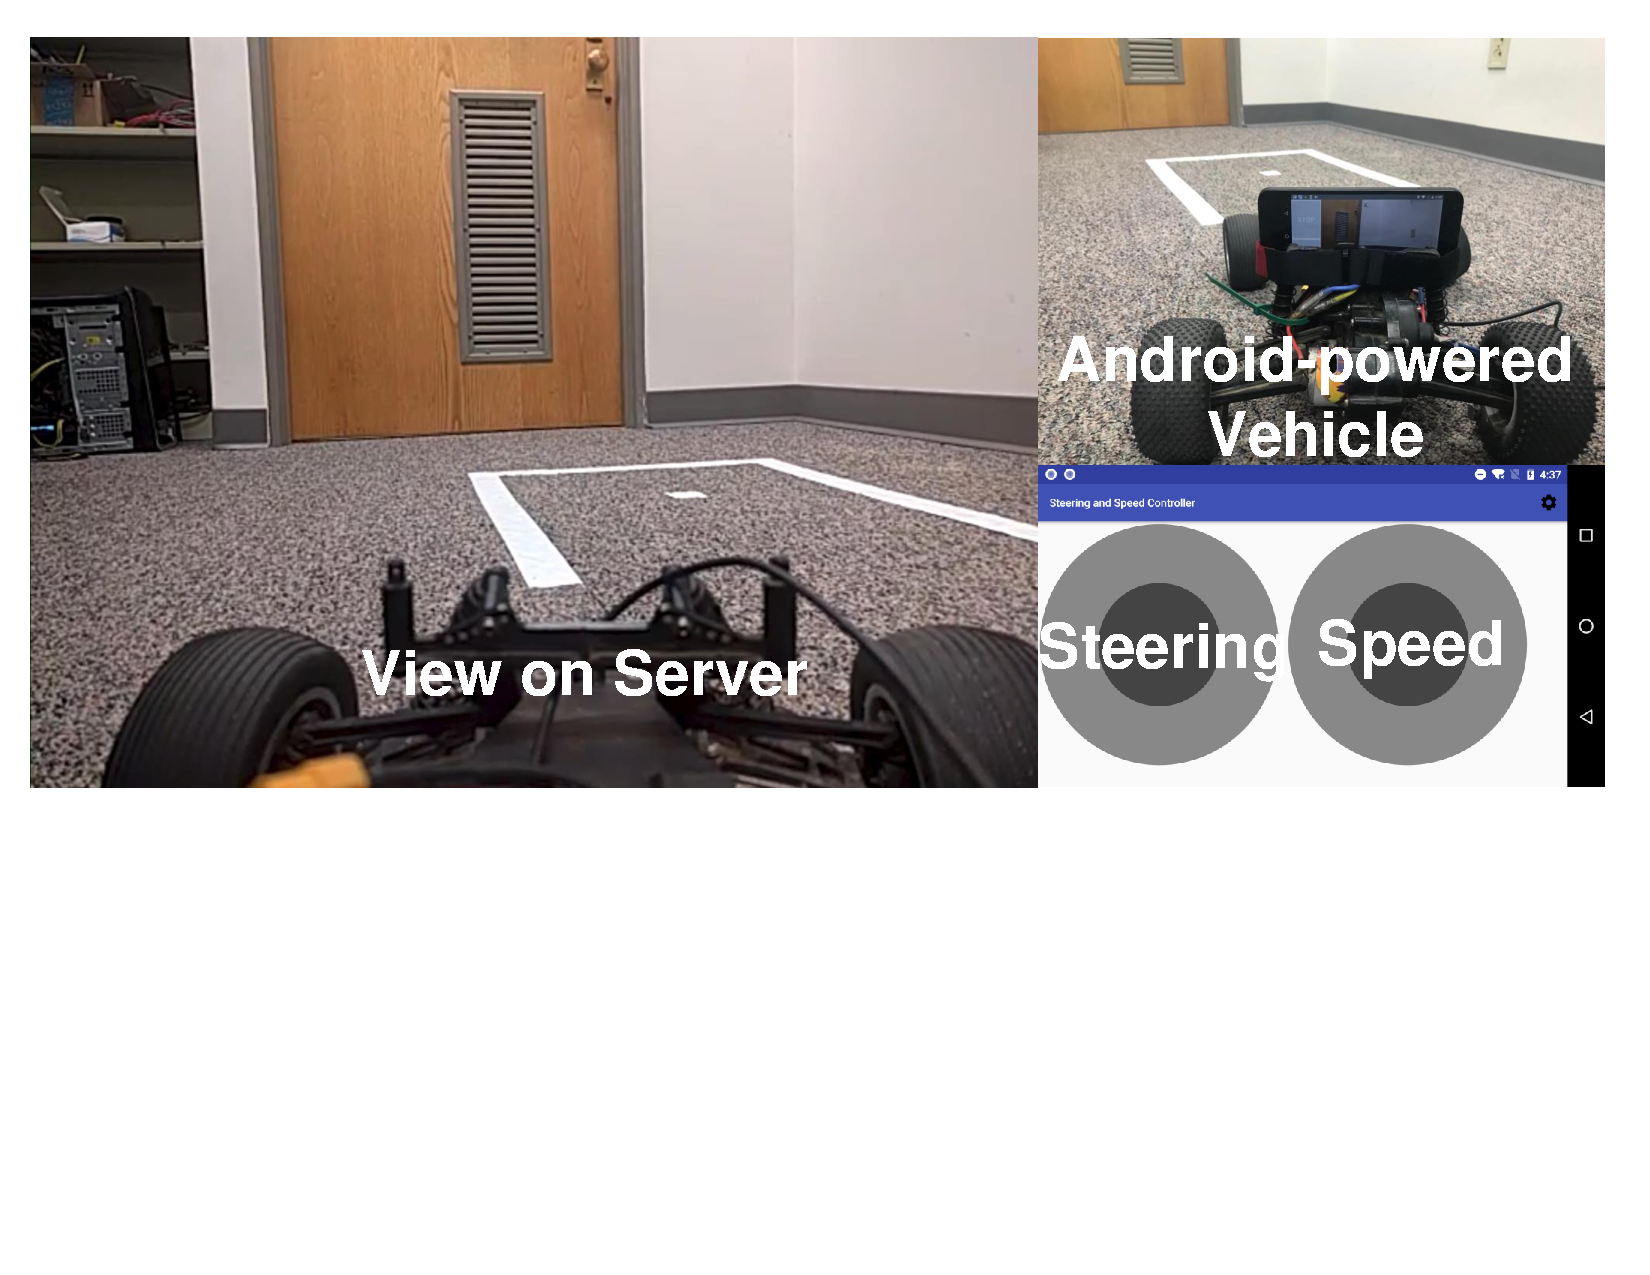
\includegraphics[width=3.0in,angle=0]{Figs/RTDrive/rc_car_cropped.pdf}
\vspace{-0.2cm}
\caption{The live streaming and remote control platform.}
\vspace{-0.2cm}
\label{platform}
\end{figure}


The framework consists of two parts, an Android-powered 
self-driving vehicle and a remote control server. 
The customized remote control vehicle
and the overview of the entire platform are illustrated in Fig. \ref{rc_vehicle} and Fig. \ref{platform}.


The self-driving and streaming client is implemented as
Android application. 
The self-driving and control app compress the video by using 
video compression standard H.264 or MPEG-4 \cite{marpe2006h}.  
Meanwhile, it identifies lane markers by using OpenCV
library and customized detection algorithms. 
The lane markers detection modules are implemented
in C/C++ and the interfaces are exported to upper 
layer through Java Native Interface (JNI).  
In the Android-powered self-driving system, 
the app transfers the control message to the
Arduino board through a Micro USB cable. 
A Hall Effect Sensor is installed to track vehicular speed
by recording the number of wheel rotations per second. 
The Arduino board bridges the Android app and the hardwares, 
i.e., the steering controller and hall effect sensor. 


The multi-thread and event-driven remote control 
server is implemented in C++.  
One UDP thread to used to receive the video stream from the
self-driving vehicle. 
The UDP thread sends the compressed video data to a GStreamer
pipeline \cite{gstreamer} running in another thread. 
The GStreamer pipeline decompresses, displays and records the video.   
There is another thread receives control message from a customized
controller to control the vehicle by human operator.


There are totally 2700+ lines of Java code for Android app implementation
and 3200+ lines of C/C++ code for the remote server.
The minimum Android SDK version is 21, which is the minimum requirement
of OpenCV3.2 SDK for Android platform. 
The Android phone we use is Nexus 5x. 
It has a reversed camera sensor and we have to rotate the camera by 180 degree
programmatically. 
The remote server is implemented on Ubuntu 16.04. 
The GStreamer version we use is 1.0. 




\section{Experimental Results}




in this section, we evaluate the context-aware encoding algorithm
and live streaming protocol. 


\begin{figure*}[ht]
  \centering
  \begin{subfigure}[t]{0.25\textwidth}
    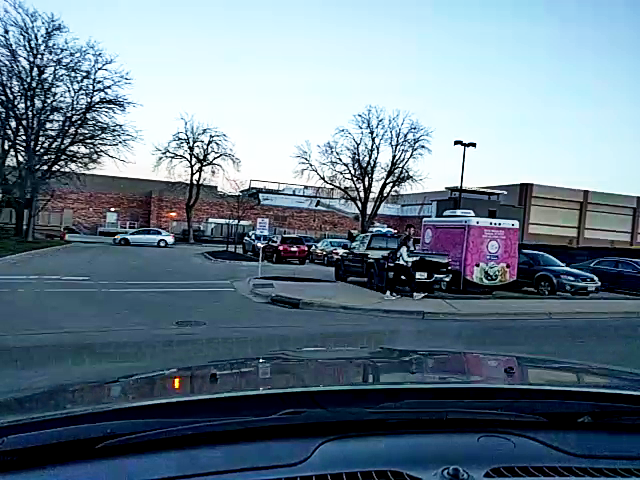
\includegraphics[width=\linewidth]{Figs/RTDrive/evaluation/frames/default_0.png}
  \end{subfigure}%
  \begin{subfigure}[t]{0.25\textwidth}
    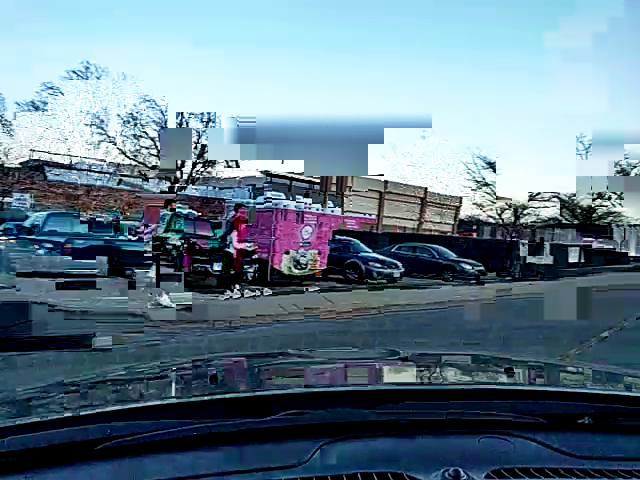
\includegraphics[width=\linewidth]{Figs/RTDrive/evaluation/frames/default_1.png}
  \end{subfigure}%
  \begin{subfigure}[t]{0.25\textwidth}
    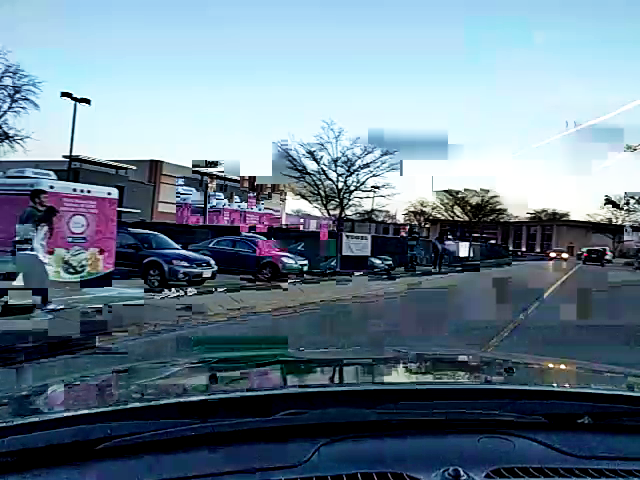
\includegraphics[width=\linewidth]{Figs/RTDrive/evaluation/frames/default_2.png}
  \end{subfigure}%
  \begin{subfigure}[t]{0.25\textwidth}
    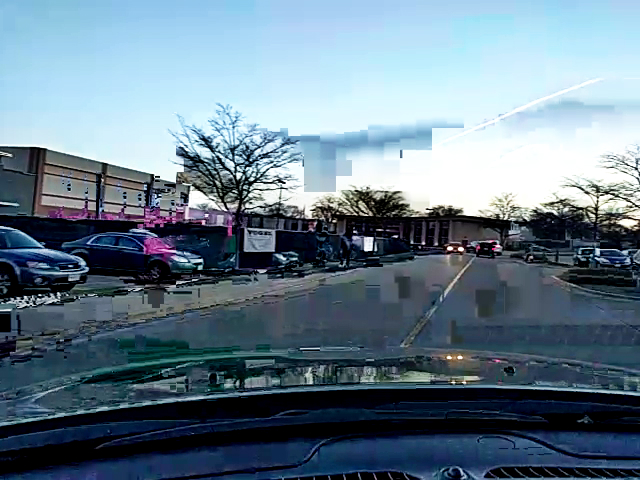
\includegraphics[width=\linewidth]{Figs/RTDrive/evaluation/frames/default_3.png}
  \end{subfigure}%
%  \begin{subfigure}[t]{0.2\textwidth}
%    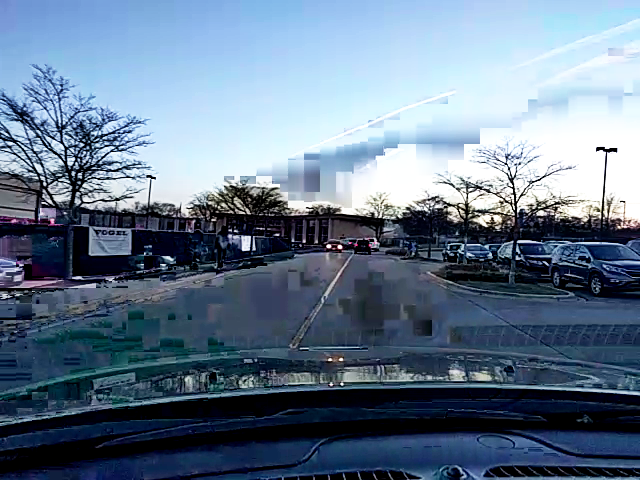
\includegraphics[width=\linewidth]{Figs/RTDrive/evaluation/frames/default_4.png}
%  \end{subfigure}%
  \label{default_encoding_images}
  
   \begin{subfigure}[t]{0.25\textwidth}
    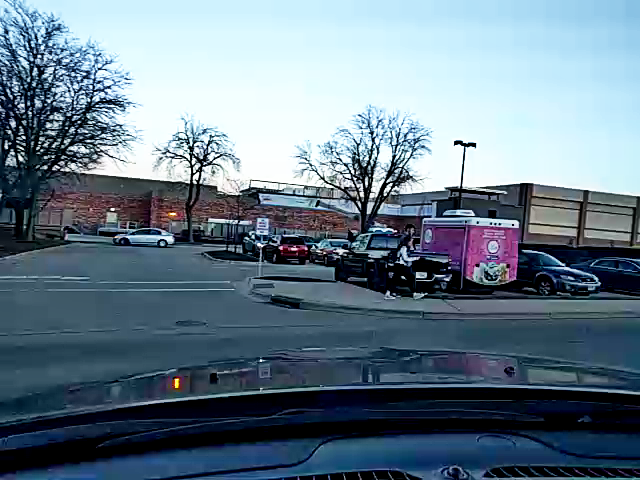
\includegraphics[width=\linewidth]{Figs/RTDrive/evaluation/frames/context_0.png}
  \end{subfigure}%
  \begin{subfigure}[t]{0.25\textwidth}
    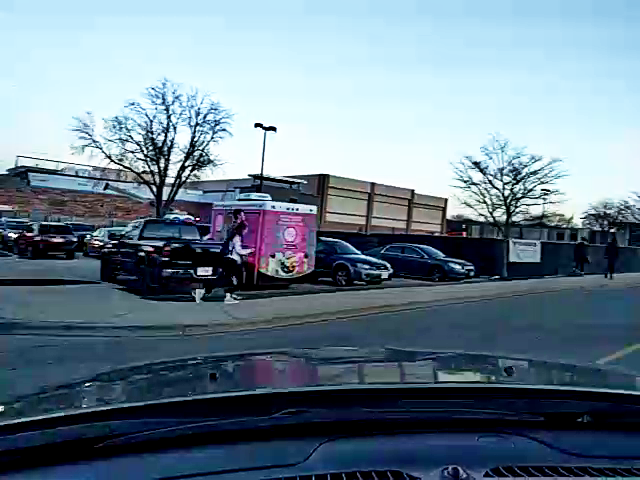
\includegraphics[width=\linewidth]{Figs/RTDrive/evaluation/frames/context_1.png}
  \end{subfigure}%
  \begin{subfigure}[t]{0.25\textwidth}
    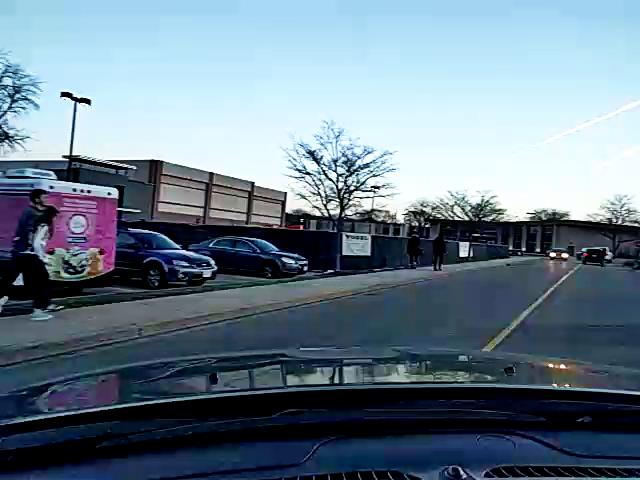
\includegraphics[width=\linewidth]{Figs/RTDrive/evaluation/frames/context_2.png}
  \end{subfigure}%
  \begin{subfigure}[t]{0.25\textwidth}
    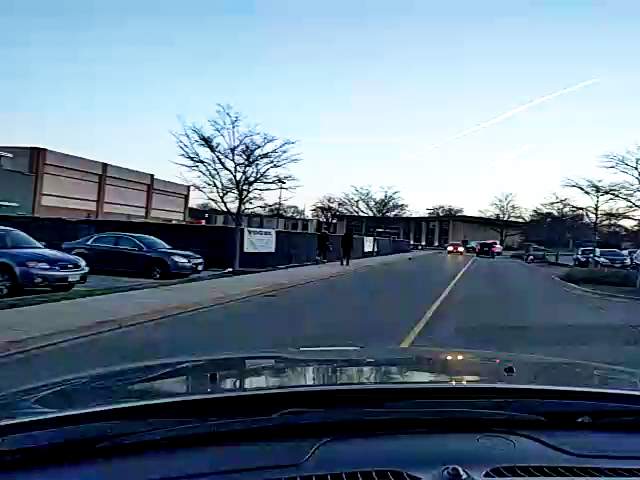
\includegraphics[width=\linewidth]{Figs/RTDrive/evaluation/frames/context_3.png}
  \end{subfigure}%
%  \begin{subfigure}[t]{0.2\textwidth}
%    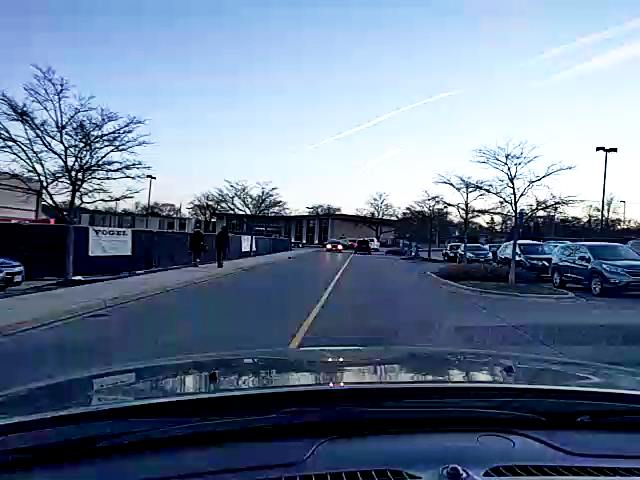
\includegraphics[width=\linewidth]{Figs/RTDrive/evaluation/frames/context_4.png}
%  \end{subfigure}%
  \caption{Images encoded by using fixed I-frame interval (above) and 
          context-aware encoding method (below) with 1mbps.
         The first frame is less clear than the default method, but the overall
         video quality is much higher. }
  \label{context_encoding_images}
\end{figure*}


\subsection{Context-Aware Video Encoding}

We compare the video quality of context-aware video encoding method 
with that of default encoding method in this section. 
We collect the raw frames under 5 different driving activities
of around 10 miles. 
The driving speed is from 0mph to 40mph and there are totally 22 
turns (exceed 60 degrees). 
At data collection time, we mount the Android phone in a vehicle
and drive the vehicle in different road segments, 
each raw frame is stored in the sdcard with predefined format. 
The raw frame data is collected through Android's \emph{onPreviewFrame}
callback function, where each captured frame is passed in 
as a byte array. 
Each raw frame starts with a fixed length header, which stores
the time and the real time sensor data. 
Each raw frame has the same size given the same resolution (640x480)
and raw frame format (Android YUV format) in a single trip. 
At evaluation time, we use Android to load in the raw frames
and encode the raw frames with different video encoding methods. 
The encoded frames are sent to the server to convert back
to the video, which is used to calculate the image quality. 


\subsubsection{Micro-benchmark}
\label{mico_context}

When load the raw frames, we encode them with context-aware video encoding
and the default H.264 video encoding, respectively. 
We use video encoding efficiency as a metric to evaluate video
encoding methods. 
We refer video encoding efficiency to video quality given the
same video encoding bitrate or the video encoding bitrate that
achieves the same video quality. 
We extract the frames when the car is marking a turn.
We replay the video by using 
the default encoding method with fixed
I-frame interval of 3s
and context-aware encoding method, 
and the sample images are shown in Fig. \ref{context_encoding_images}.
For the images with fixed I-frame
interval (above), 
all the images are blurred and distorted except for the first image (I-frame). 
For the images with context-aware encoding method (below),
all the images are with good quality.  

\subsubsection{Parameter Selection}
\label{sec_selection}


\begin{figure}[ht]
\centering
  \begin{subfigure}[t]{0.24\textwidth}
    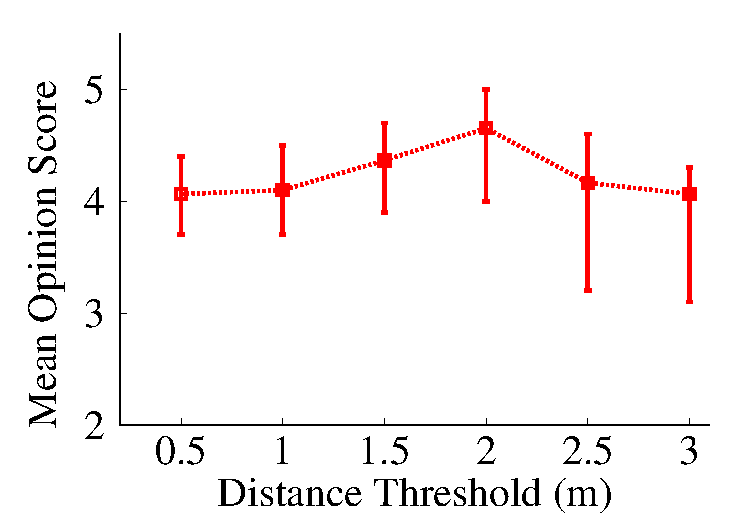
\includegraphics[width=\linewidth]{Figs/RTDrive/evaluation/context_dist.pdf}
    \vspace{-0.5cm}
    \caption{Distance threshold.}
    \label{param_dist}
  \end{subfigure}%
  \begin{subfigure}[t]{0.24\textwidth}
    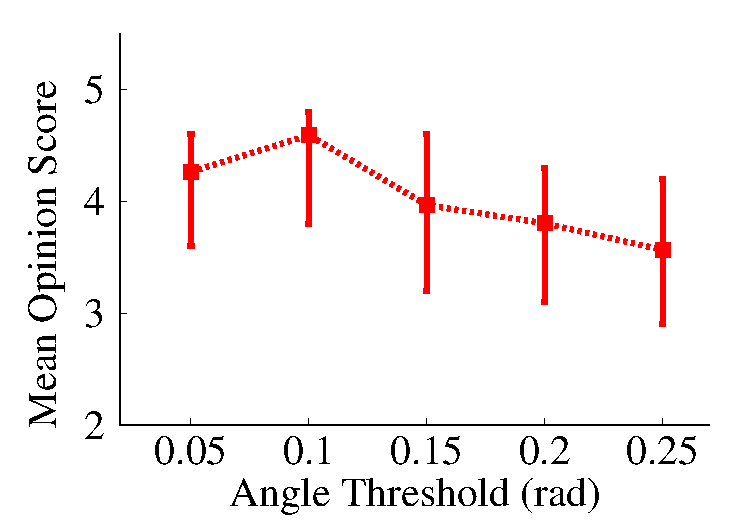
\includegraphics[width=\linewidth]{Figs/RTDrive/evaluation/context_gyro.pdf}
    \vspace{-0.5cm}
    \caption{Angle threshold.}
    \label{param_angle}
  \end{subfigure}%
  \vspace{-0.2cm}
  \caption{Sensitivity to parameters. }
  \label{parameters}
  \vspace{-0.25cm}
\centering
\end{figure}


The performance context-aware video encoding method depends on
two parameters, the distance and angular velocity thresholds.
The threshold is used to control how frequent the video 
encoder produces a I-frame. 
A lower threshold produces more I-frames and a higher
threshold produces more P-frames. 
To select the threshold parameters, we repeat the 
experiments in section \ref{mico_context} with different 
threshold settings.
We divided the trips into straight road and turns, 
and test different distance threshold on straight roads and
different angular velocity threshold in turns. 
The results are shown in Fig. \ref{parameters}. 
A high distance/angle threshold means there will be less 
I-frames (or a larger I-frame interval) and the frame quality heavily depends 
on the qualities of previous frames. 
As discussed in section \ref{sec_frame_encoding}, 
a large I-frame interval may cause bad quality P-frames 
when the scene changes frequently, 
which causes poor tail quality when using higher
thresholds. 

\subsubsection{Overall Performance}



\begin{figure}[t]
\centering
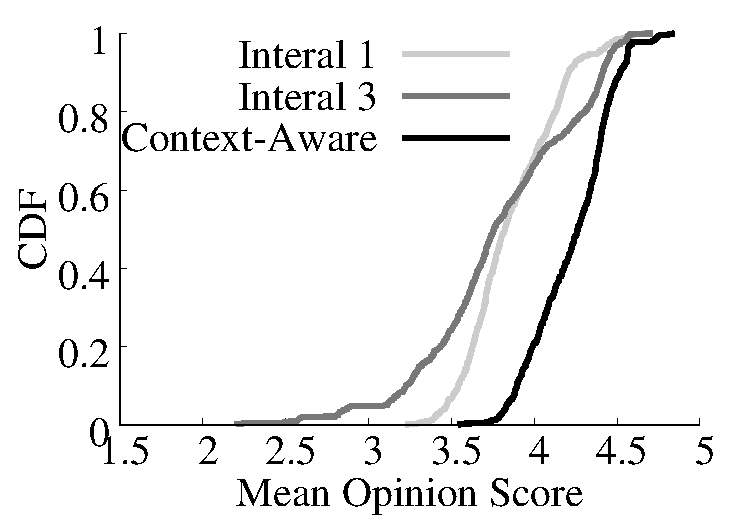
\includegraphics[width=2.8in,angle=0]{Figs/RTDrive/evaluation/context_quality.pdf}
\caption{Video quality under default encoding method
and context-aware encoding method.}
\vspace{-0.2cm}
\label{context_quality}
\centering
\end{figure}


The overall performance of context-aware video encoding method is evaluated
through all the 5 trips we collected. 
We use the parameter settings selected in section \ref{sec_selection}.
The default comparison method uses a fixed I-frame interval of 1s and 3s.
As shown in Fig. \ref{context_quality}, 
if we use a small I-frame interval (1s in this case), the deviation of the image
qualities are small while the average qualities are dropped
as the frame differences are not fully utilized. 
If we use a larger I-frame interval (3s in this case), 
the deviation of the image qualities are larger while some I-frames
have better quality than the rest.
Context-aware encoding is able to select I-frame and P-frame
based on potential frame difference changes, 
which lead better overall performance than using
fixed interval encoding method.  

\subsection{Consistent-Latency Remote Control}


\begin{figure*}[ht]
  \begin{subfigure}[t]{0.20\textwidth}
    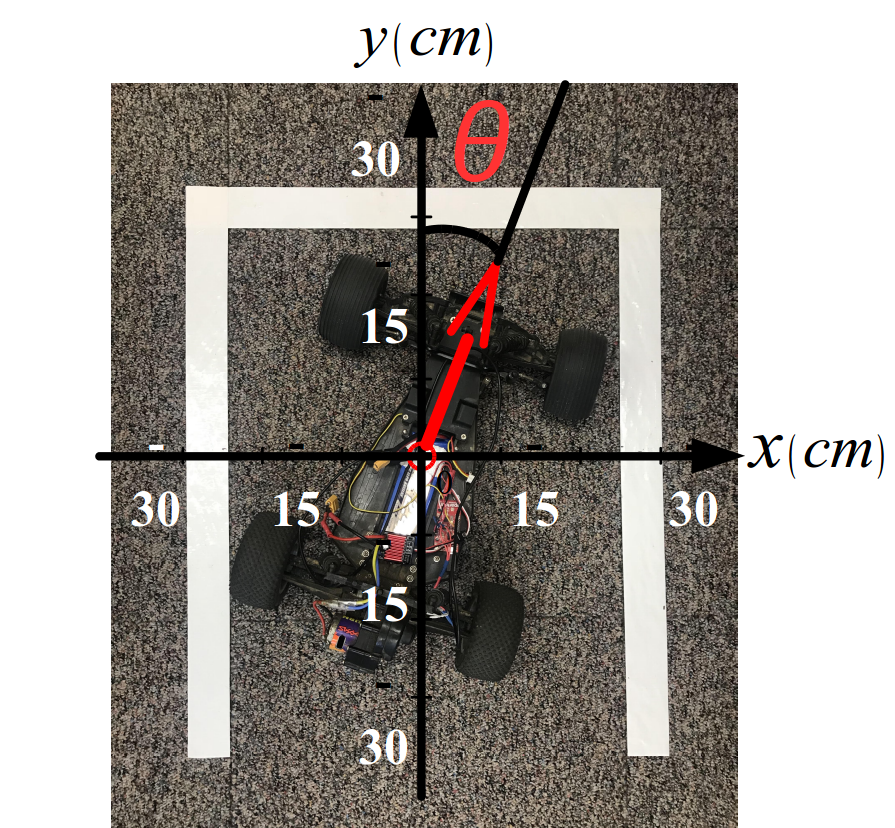
\includegraphics[width=\linewidth]{Figs/RTDrive/evaluation/car.png}
    \caption{Parking spot.}
    \label{parking_car}
  \end{subfigure}
  \begin{subfigure}[t]{0.26\textwidth}
    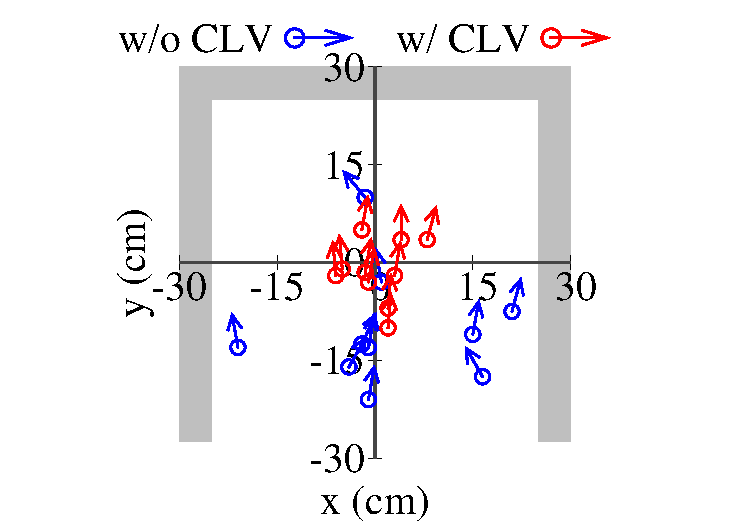
\includegraphics[width=\linewidth]{Figs/RTDrive/evaluation/position_fewerpoints.pdf}
    \caption{Parking control illustration.}
    \label{consistent:illustration}
  \end{subfigure}%
  \begin{subfigure}[t]{0.26\textwidth}
    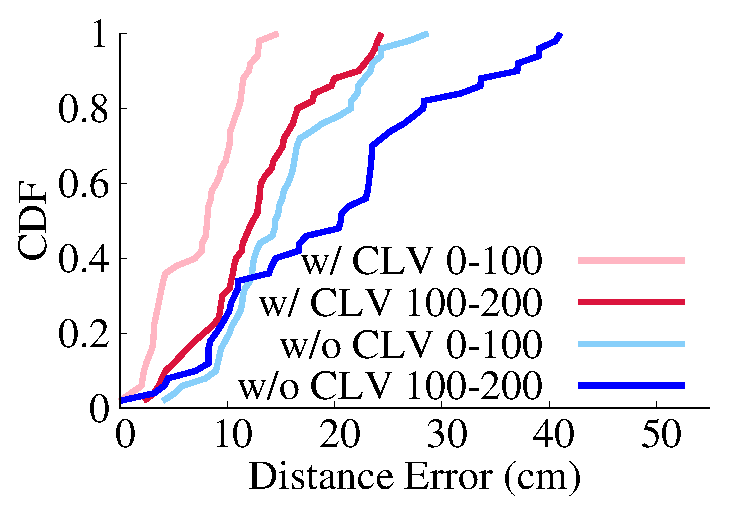
\includegraphics[width=\linewidth]{Figs/RTDrive/evaluation/Distance.pdf}
    \caption{Parking distance error.}
    \label{consistent:distance}
  \end{subfigure}%
  \begin{subfigure}[t]{0.26\textwidth}
    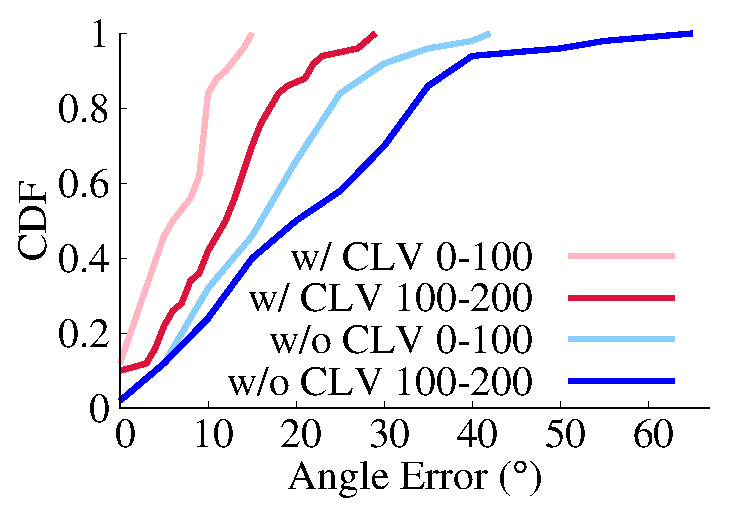
\includegraphics[width=\linewidth]{Figs/RTDrive/evaluation/Angle.pdf}
    \caption{Parking angle error.}
    \label{consistent:angle}
  \end{subfigure}%
  \caption{The precision of remote control of different operators under 
various latency settings.}
  \label{feasibility}
  \vspace{-0.2cm}
\end{figure*}


To understand the impact of consistent-latency on
steering and speed control of the vehicle, 
we conduct user study on a parking task.
Parking is one of most challenging driving activities, 
and a parking lot experiment can test the most fundamental 
controls of vehicle of the operators, steering and speed.
This experiment is conducted under indoor Wi-Fi environment. 
 
As shown in Fig. \ref{parking_car}, 
we draw a parking spot on the ground by using white tapes.
The remote control car is 5 meters vertical distance and 1 meter horizontal distance away. 
The operators are asked to drive the car by using
steering and forwarding control.
The backward control is disabled so that the operator has no
chance to do readjustment and the operator
has only one chance to park the car in the spot.   
The operators can only see the live streaming video on the server monitor. 
The whole setup is similar to a car racing game, except
the operator is controlling a real car. 


The participates start with 10 test drives to get familiar with 
the environment and get feedback themselves for their
control precision and parking performance. 
After the test drive, they are asked to drive the car under
different latency and parameter settings. 
The experiment consists of 20 groups with extra latency
of 0ms, 40ms, 80ms, 120ms, 160ms and 200ms. 
Half of the experiment groups are conducted with consistent-latency
enabled and half are not.
The experiment are randomly generated and the participants
do not know the settings at the time they control the vehicle. 


We use distance error and angle error to evaluate
parking performance. 
Distance error refers to the distance of the parked car to the distance
of the center of the parking spot. 
Angle error refers to te difference between the parked direction and vertical direction.
We divide the results into two latency groups, 0-100ms and 100-200ms. 
With CLV, the both the median distance error and median angle error
are reduced by half under different latency settings. 
The parking performance of one participate under 80ms latency is shown
in Fig. \ref{consistent:illustration}. 
In the cases there is no CLV, the video frames may be lagged or jumped due to
the variance of wireless network latency and bandwidth. 
With CLV, the participates have smoother view, so that 
the control can be more precise as they can 
``predict'' the impact of the latency. 



\subsection{Live Streaming Protocol}

We evaluate the live streaming protocol in this section. 
We compare the performance of UDP and TCP, with and without
FEC. 
We also present performance of bandwidth and loss rate
estimation module of the protocol. 

\subsubsection{FEC and Video Quality}

\begin{figure}[t]
\centering
\vspace{-0.3cm}
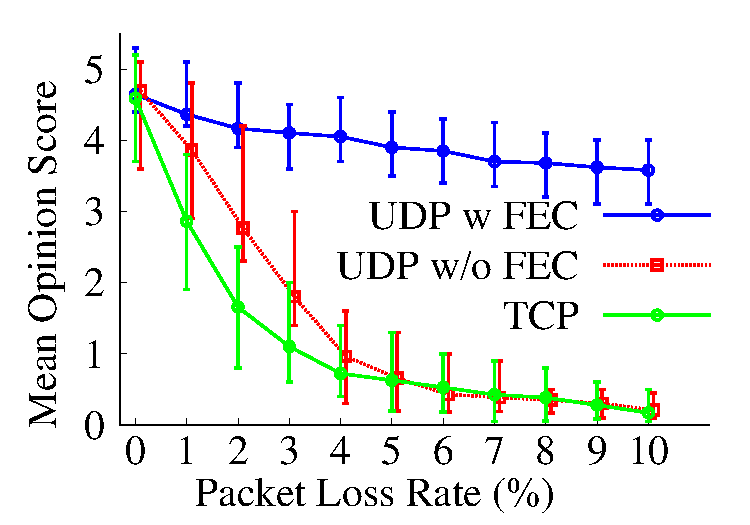
\includegraphics[width=2.6in,angle=0]{Figs/RTDrive/evaluation/video_quality_errorbars.pdf}
\vspace{-0.3cm}
\caption{Video quality under different loss rates.}
\vspace{-0.2cm}
\label{loss_quality}
\centering
\end{figure}


\begin{figure*}[ht]
\centering
  \begin{subfigure}[t]{0.33\textwidth}
    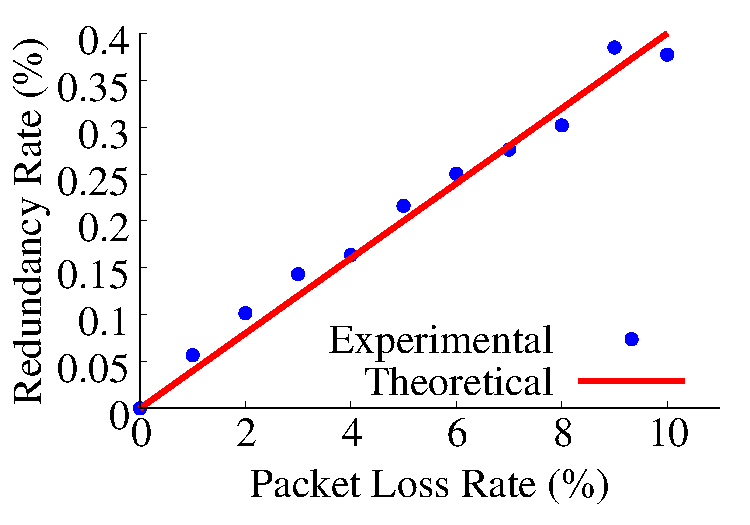
\includegraphics[width=\linewidth]{Figs/RTDrive/evaluation/fec_ratio.pdf}
    \vspace{-0.5cm}
    \caption{FEC ratio under various loss rate.}
    \label{fec_ratio}
  \end{subfigure}%
  \begin{subfigure}[t]{0.33\textwidth}
    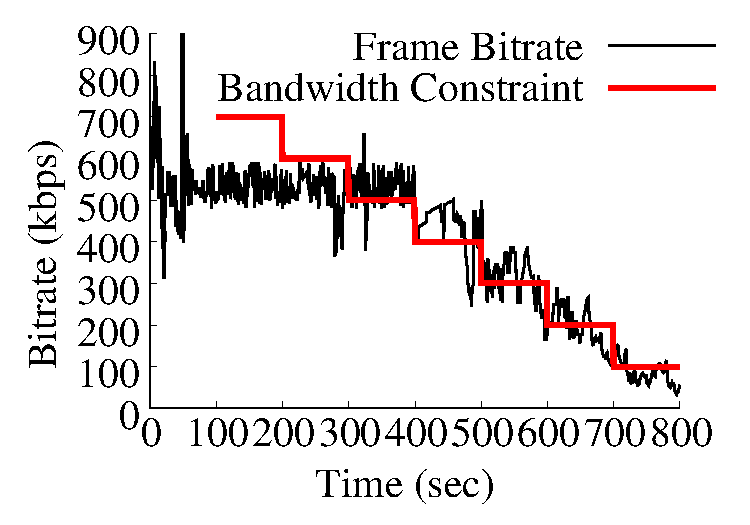
\includegraphics[width=\linewidth]{Figs/RTDrive/evaluation/bandwidth.pdf}
    \vspace{-0.5cm}
    \caption{Bandwidth estimation and adaptation.}
    \label{bandwidth}
  \end{subfigure}%
  \begin{subfigure}[t]{0.33\textwidth}
    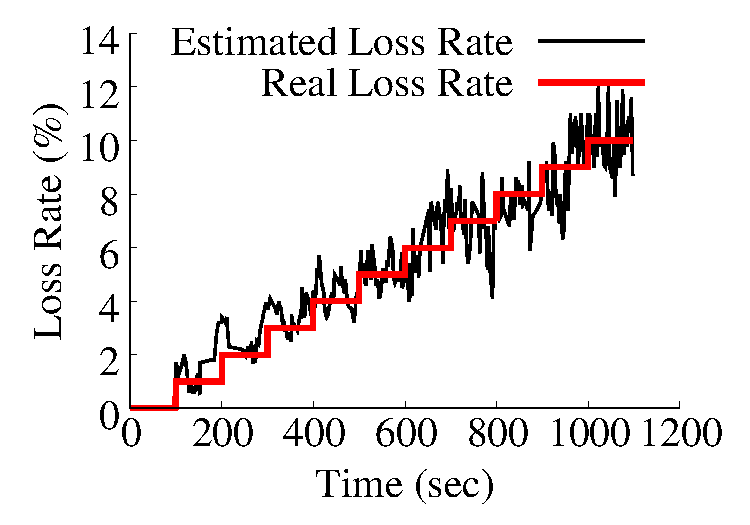
\includegraphics[width=\linewidth]{Figs/RTDrive/evaluation/lossrate.pdf}
    \vspace{-0.5cm}
    \caption{Loss rate estimation.}
    \label{loss_rate}
  \end{subfigure}%
  \vspace{-0.3cm}
  \caption{Estimation accuracy of transmission protocols. }
  \label{feasibility}
  \vspace{-0.2cm}
\centering
\end{figure*}



We evaluate the impact of packet loss rate on video quality, 
with and without FEC, respectively. 
We use the Android app to record and stream a driving video 
we recorded for trace replay experiments. 
The server connects with the router through a Ethernet 
cable and the Android connects with the same router
through Wi-Fi.  
The server will store the streaming video locally
and then use the video quality check tool 
to calculate the quality. 
The results are shown in Fig. \ref{loss_quality}. 
If there is no FEC or similar redundancy mechanism, 
a loss rate of 3\% makes most frames distorted and hard to view. 
Video encoding algorithm is sensitive to packet loss. 
If one fraction of a I-frame get lost, that fraction
cannot be displayed properly. 
Also, the quality of the following P-frame will be even worse 
since the compression relies on the missing fraction 
and the video decoder cannot recover properly. 
The future P-frame which relies on previous I-frame
and P-frame will have even worse quality for
the same reason. 
The loss of one fraction will propagate to all of the 
following P-frames.  
With FEC encoding, the server side can recover most of the 
frames. 


\subsubsection{UDP and TCP}


We perform a comparative benchmark of UDP and TCP under various 
loss rate, and the results are shown in Fig. \ref{loss_quality}. 
Other modules are using the default settings. 
In UDP measurement, the FEC is enabled for fair
comparison. 
In TCP measurement, the FEC is disabled since
TCP is lossless protocol. 
Unlike TCP, the latency of UDP is insensitive to packet loss. 
As shown in Fig. \ref{loss_quality}, the latency of UDP is not sensitive
to packet loss as the transmission rate is smaller
than available bandwidth. 
TCP is sensitive to packet loss, as TCP will treat packet loss
as congestion and then try to slow down transmission by 
The higher latency of TCP at higher loss rate is caused by 
two reasons. 
First, if one frame packet is lost, then the whole frame has to
wait for the retransmission of that packet, 
which cause an extra RTT. 
Second, the TCP congestion control will slow down future transmission
upon packet loss, which increase the buffering time of 
future frames. 
Under loss rate of more than 2\%, the streaming video will freeze
frequently and cause the video not able to view. 



\subsubsection{Bandwidth and Packet Loss Rate Estimation}

To evaluate how our live streaming protocol performs under 
different wireless network conditions, 
we emulate various loss and latency under indoor Wi-Fi
environments.  
We use netem and Intermediate Functional Block pseudo-device \cite{netem} to 
create loss, extra network delay and bandwidth constraints. 
In this experiment, we add constraints on the bandwidth of the 
Ethernet port of the server. 
The server connects with the router with an Ethernet cable. 
The Android connects with the router through Wi-Fi. 
We decrease the bandwidth constraints from $700kbps$ to $100kbps$. 
The Android streams the video to the server and adapt 
the video bitrate according to the estimation and adaptation algorithm
described in section \label{sec_bandwidth}. 
Similar to bandwidth constraint, we set packet loss rate by using 
netem \cite{netem}. 
The loss rate estimation result is shown in Fig. \ref{loss_rate}. 
We increase the loss rate 1\% for every 100s, 
and our protocol can track packet loss rate closely. 


\subsubsection{End-to-End Latency Breakdown}


\begin{table*}[t]
  \centering
  \caption[latency]{Latency Breakdown}
  \vspace{-0.0cm}
  \label{latency}
  \begin{tabular}{|c|c|c|c|c|c|c|}
  \hline
Modules & Lane Detector & Object Detector  &  Frame Encoding  &  Serial & Wireless Network  & End-to-end  
\\  \hline
Latency & 38ms & 30ms & 21-42ms & 2-10ms & 40-200ms & 200-500ms
\\  \hline      
  \end{tabular}
  \vspace{-0.0cm}
\end{table*}


\begin{figure}[t]
\centering
\vspace{-0.0cm}
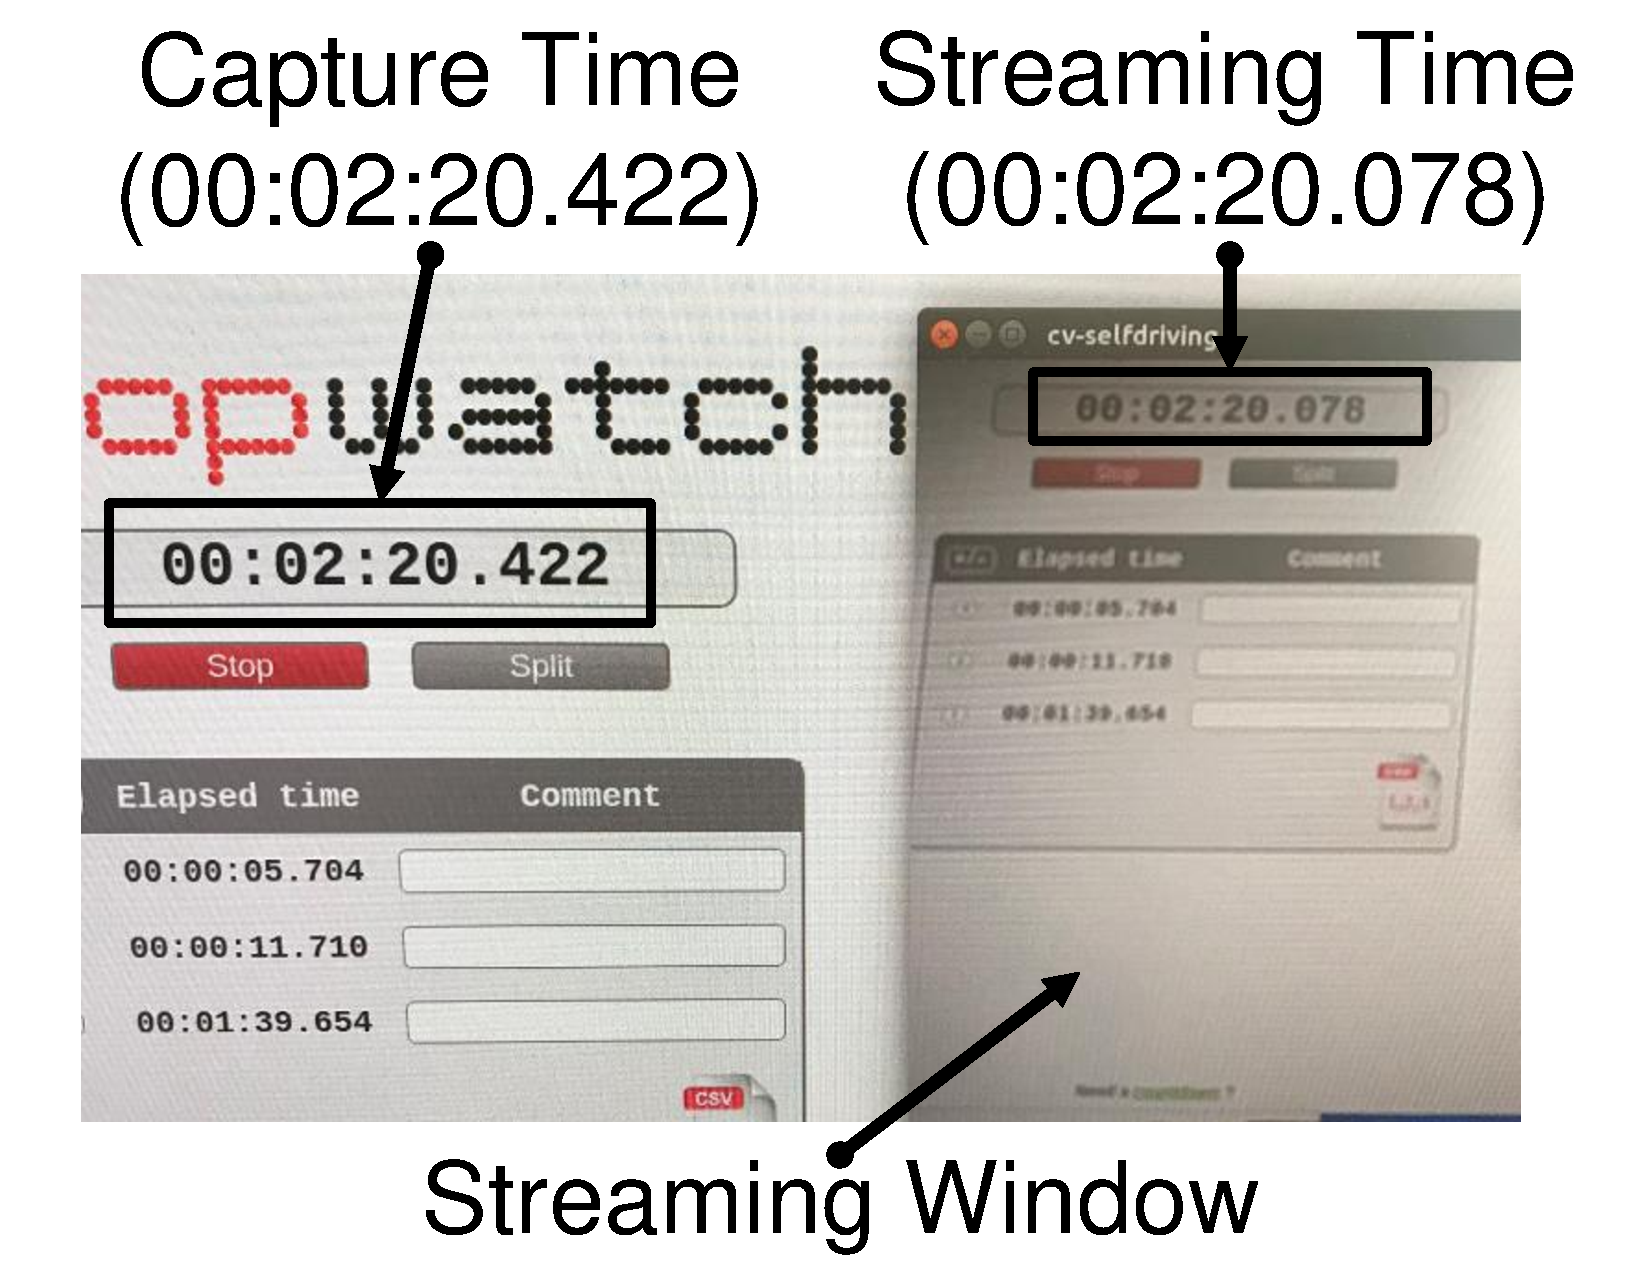
\includegraphics[width=2.4in,angle=0]{Figs/RTDrive/evaluation/endtoend.pdf}
\vspace{-0.2cm}
\caption{The end-to-end streaming and display latency measurement.}
\vspace{-0.2cm}
\label{endtoend}
\centering
\end{figure}


We benchmark the latency of each module and summarize the 
results in Table \ref{latency}. 
The latency of lane detector, frame encoding and FEC are measured
in the Android app. 
Each module is called through a API function. 
A timer recorded the timestamp both before and after calling this function and 
the difference is the latency caused by this module. 
It should be noted that object identification can be separated 
into another thread to reduce the streaming latency, 
and we left such optimization and the evaluation into future work.  
The round-trip latency of serial communication between Android device and 
Arduino board is measured by message with timestamp.  
The round-trip latency is frame latency measured by packet timestamps. 
End-to-end latency is the latency between the time the frame is captured
and the time the frame is viewed by user through streaming. 
To measure the end-to-end latency, we start a millisecond timer
on the server, and use the Android device to stream the 
timer to the same screen. 
As shown in Fig. \ref{endtoend}, we take the screenshot of 
the streaming window as well as the timer.
The streaming window is the video display on the server for the
streaming videos from the Android device. 
The difference between the two timer is the end-to-end latency
for video streaming.  
We illustrate that it suffers 200-500ms end-to-end display latency 
when streaming 640x480 resolution frames by using
standard video compression algorithms \cite{marpe2006h}
under current LTE networks. 
Compared with average driver reaction time of 0.7-2.4 seconds \cite{taoka1989brake}, 
the extra delay is tolerable for human operator
to control the car remotely.  

To reduce the end-to-end streaming latency, there are several techniques 
can be used. 
A higher performance system board can be used to replace the Android phone. 
Some optimization techniques such as \cite{likamwa2015starfish} can be used
to avoid duplicate operations and reduce image processing latency. 
The video encoding speed can be improved by dedicated hardware and
the wireless communication speed can also be improved. 
In the Wi-Fi setting, the Android Wi-Fi module enters sleep state
every 100ms, even the highest performance is enabled. 
Such sleep state causes 50-100ms one-way latency. 
Also, 5G and/or better designed wireless communication infrastructure and protocol
can be used to reduce the communication latency. 






\section{Summary of RTDrive}


This chapter introduces RTDrive, a real-time live streaming and 
remote control framework to augment self-driving
systems upon occasional system failures. 
RTDrive consists of an Android-powered self-driving
and video streaming system and a server that can
display the camera view streamed in real time 
and send back control command to control the
vehicle. 
RTDrive includes some system modules 
such as video encoding/decoding, FEC encoding/decoding,
loss rate and bandwidth estimation, vehicle dynamics
sensing, as well as transportation protocols. 
Such a framework facilitate future research topcis such as
video encoding and streaming, video bitrate adaptations
in this application domain. 
Based on this framework, 
we design and implement several innovative mechanisms to improve
video encoding efficiency and user viewing experience.
We introduce a context-aware video encoding technique
to encode video based on vehicle dynamics, 
which improves video encoding efficiency by 10\%-30\%
through real world driving trace replay,
and consistent-latency to improve user viewing experience
by reducing lags, which improves user control
precision by 2x through user study. 
 








\begin{enumerate}
  \begin{algorithm}[H]
   \caption{FEC Packets Buffering}
    \label{fec_buffer}
    \begin{algorithmic}[1]
\Function{buffering}{$buffer, curid, pkt$}
\Comment{Where buffer - Packet buffer for decoding, 
curid - latest frame identifier, 
pkt - Frame packet}
  \State ${id} = pkt.id$
  \State ${k} = pkt.k$
  \If {$curid < id$}
    \State \Return
  \EndIf
  \If {$curid == id$}
    \State $buffer.insert(pkt)$
    \If {$buffer.size() == k$}
      \State $decodePackets(buffer)$
      \State $buffer.clear()$
      \State $curid = curid + 1$
    \EndIf
  \Else
    \If {$buffer.size() > 0$}
      \State $decodePackets(buffer)$
    \EndIf
    \State $buffer.clear()$
    \State $buffer.insert(pkt)$    
    \State $curid = id$
  \EndIf
\EndFunction
\end{algorithmic}
\end{algorithm}
\end{enumerate}






